% ============================================
% Risk-Sensitive Credit Card Default Prediction
% A Machine Learning Approach with
% Repayment-Behavior Feature Engineering
% ============================================
\documentclass[conference]{IEEEtran}
\usepackage{cite}
\usepackage{amsmath,amssymb,amsfonts}
\usepackage{graphicx}
\usepackage{booktabs}
\usepackage{array}
\usepackage{hyperref}
\usepackage{float}


\hypersetup{
    colorlinks=true,
    linkcolor=black,
    citecolor=black,
    urlcolor=blue
}

% Decimal-aligned columns
\newcolumntype{d}[1]{D{.}{.}{#1}}

\graphicspath{{outputs/modeling_figures/}{outputs/results/}{code/EDA/}}

\begin{document}

\title{Risk-Sensitive Credit Card Default Prediction: A Machine Learning Approach with Repayment-Behavior Feature Engineering}

\author{
    \IEEEauthorblockN{Your Name}
    \IEEEauthorblockA{Data Science\\
    BNU-HKBU United International College\\
    Zhuhai, China\\
    email@mail.uic.edu.hk}
}

\maketitle

\begin{abstract}
Credit card default prediction is a critical task for financial risk management, yet standard classification approaches often overlook the inherent class imbalance and treat the problem as a simple accuracy-oriented binary classification task. In this paper, we extend credit card default prediction to a risk-sensitive prediction problem through systematic feature engineering and comprehensive model comparison. Using the UCI Credit Card dataset with 30,000 client records, we construct repayment-behavior features that capture clients' historical payment patterns, achieving significant improvements over raw features alone. We evaluate seven machine learning models---Logistic Regression, Decision Tree, KNN, SVM, Random Forest, Gradient Boosting, and XGBoost---alongside a Deep Neural Network (DNN) with focal loss optimization. Our results demonstrate that ensemble methods, particularly Random Forest (F1-score: 0.543, ROC-AUC: 0.779) and XGBoost (F1-score: 0.534, ROC-AUC: 0.772), achieve the best predictive performance. The DNN with weighted binary cross-entropy loss achieves an F1-score of 0.536, representing a 5.9 percentage point improvement over the standard DNN baseline. We further show that threshold optimization provides practical flexibility for risk-sensitive deployment scenarios.
\end{abstract}

\begin{IEEEkeywords}
Credit card default prediction, machine learning, feature engineering, class imbalance, deep neural network
\end{IEEEkeywords}

\section{Introduction}
The accurate prediction of credit card defaults is a fundamental challenge in financial risk management. Financial institutions rely on default prediction models to assess borrower risk, determine credit limits, and allocate collection resources effectively. However, this task presents several inherent difficulties: the dataset is typically imbalanced (with defaulters comprising a minority of clients), the decision boundary between defaulters and non-defaulters is often subtle, and the cost of misclassification varies depending on the stakeholder's perspective.

In this paper, we present a comprehensive machine learning framework for credit card default prediction. Our key contributions are:

\begin{enumerate}
    \item \textbf{Repayment-behavior feature engineering:} We construct 17 behavioral features that summarize clients' historical repayment patterns, demonstrating that these engineered features consistently improve model performance across all classifiers.
    \item \textbf{Comprehensive model comparison:} We systematically evaluate seven machine learning models and a deep neural network, assessing performance across multiple metrics.
    \item \textbf{Deep neural network optimization:} We investigate focal loss and weighted cross-entropy loss functions to address class imbalance, achieving a 5.9~pp improvement in F1-score over the standard DNN baseline.
    \item \textbf{Risk-sensitive threshold analysis:} We demonstrate that adjusting the decision threshold can significantly improve recall for the default class, providing practical guidance for deployment.
\end{enumerate}

The remainder of this paper is organized as follows: Section~II reviews related work. Section~III describes the dataset and exploratory data analysis. Section~IV details our methodology. Section~V presents experimental results. Section~VI discusses key findings, and Section~VII concludes the paper.

\section{Related Work}

\subsection{Credit Scoring and Default Prediction}
Credit scoring has been a central topic in financial risk management for decades. Early approaches relied primarily on linear discriminant analysis and logistic regression~\cite{hand2005good}, valued for their interpretability and regulatory compliance. As computational power increased, more sophisticated methods emerged. West~\cite{west2000neural} conducted one of the first comprehensive comparisons of neural network architectures for credit scoring, finding that properly regularized networks could outperform traditional methods.

Ensemble methods such as Random Forest~\cite{breiman2001random} and XGBoost~\cite{chen2016xgboost} have become dominant in credit risk applications due to their ability to capture non-linear relationships. Yeh and Lien~\cite{yeh2009comparisons} specifically compared data mining techniques on the same UCI Credit Card dataset used in this study, establishing a performance baseline. More recently, deep learning approaches for tabular data have gained traction. Arik and Pfister~\cite{arik2021tabnet} proposed TabNet, an attentive interpretable tabular network that uses sequential attention to select features for reasoning, achieving competitive performance on various tabular benchmarks. However, Gorishniy et al.~\cite{gorishniy2021revisiting} demonstrated that well-tuned gradient-boosted trees still outperform sophisticated deep learning architectures on most tabular data tasks, a finding that motivates our inclusion of both tree-based ensembles and DNNs in a unified comparison framework.

\subsection{Class Imbalance in Financial Data}
Class imbalance is a pervasive challenge in credit default prediction, as defaulting clients typically constitute a small minority (15\%--25\%) of the population. Standard accuracy-oriented training tends to produce models that perform well on the majority class while failing to identify high-risk defaulters. Several comprehensive surveys have characterized this problem: He and Garcia~\cite{he2009learning} provided a foundational taxonomy of imbalance learning methods, while more recent work by Krawczyk~\cite{krawczyk2016learning} surveyed emerging directions including cost-sensitive learning and ensemble approaches for imbalanced streams.

At the data level, SMOTE~\cite{chawla2002smote} generates synthetic examples of the minority class. At the algorithm level, cost-sensitive learning assigns higher misclassification costs to the minority class~\cite{elkan2001foundations}. In the deep learning domain, Focal Loss~\cite{lin2017focal} was originally proposed for dense object detection but has been adapted to binary classification with extreme imbalance. It operates by down-weighting well-classified examples via a modulating factor $(1-p_t)^\gamma$, forcing the model to focus on hard, misclassified instances. To our knowledge, the application of focal loss to credit card default prediction with deep neural networks remains underexplored, providing the primary motivation for our DNN optimization experiments.

\subsection{Feature Engineering for Credit Risk}
While raw credit data typically includes basic payment history and demographics, research has emphasized the importance of engineered features. Hand and Henley~\cite{hand2005good} discussed how behavioral features—payment-to-bill ratios, delinquency frequency, and credit utilization—capture risk signals more effectively than individual raw variables. Khandani et al.~\cite{khandani2010customer} demonstrated that machine learning models using constructed behavioral features significantly improve early warning system performance for consumer credit risk. Our work extends this direction by constructing 17 repayment-behavior features summarizing six months of payment history.

\section{Dataset and Exploratory Data Analysis}

\subsection{Dataset Description}
We use the UCI Credit Card Default dataset~\cite{yeh2009comparisons}, which contains payment records of 30,000 credit card clients from a major Taiwanese financial institution from April to September 2005. Each record includes 23 features spanning four categories:

\begin{itemize}
    \item \textbf{Demographic variables:} LIMIT\_BAL (credit limit), SEX, EDUCATION, MARRIAGE, AGE
    \item \textbf{Repayment status:} PAY\_0 to PAY\_6 (monthly repayment status)
    \item \textbf{Bill amount:} BILL\_AMT1 to BILL\_AMT6 (monthly bill statements)
    \item \textbf{Payment amount:} PAY\_AMT1 to PAY\_AMT6 (monthly payment amounts)
\end{itemize}

The target variable indicates whether the client defaulted in October 2005. The dataset contains no missing values or duplicate records.

\begin{figure}[H]
    \centering
    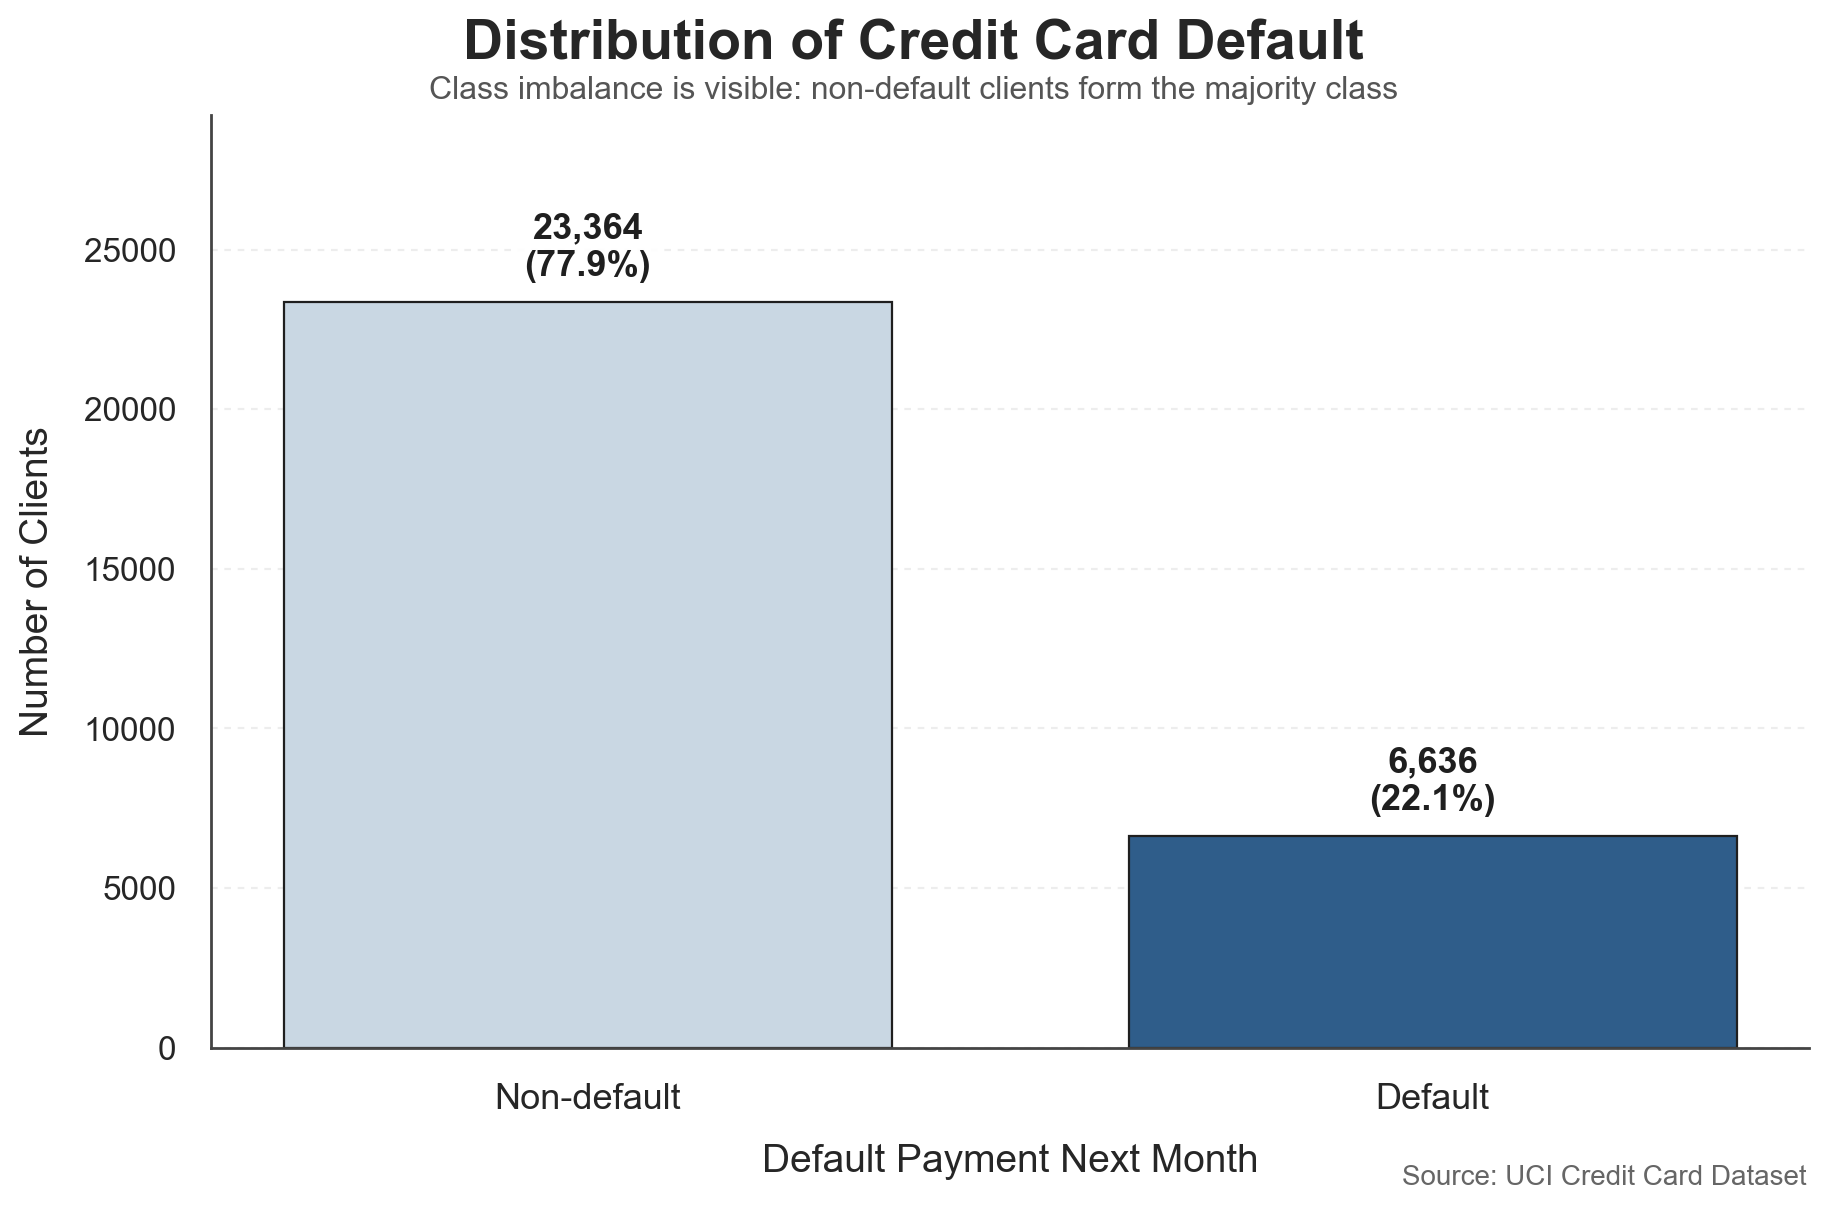
\includegraphics[width=0.45\textwidth]{01_target_distribution_refined.png}
    \caption{Distribution of the target variable: 77.9\% non-default versus 22.1\% default}
    \label{fig:target_dist}
\end{figure}

\subsection{Feature Correlation Analysis}
To understand the relationships among features and their predictive power, we computed Pearson correlation coefficients. Figure~\ref{fig:corr_heatmap} presents the full feature correlation heatmap, and Fig.~\ref{fig:behavior_corr} highlights correlations between engineered features and the default target.

\begin{figure}[H]
    \centering
    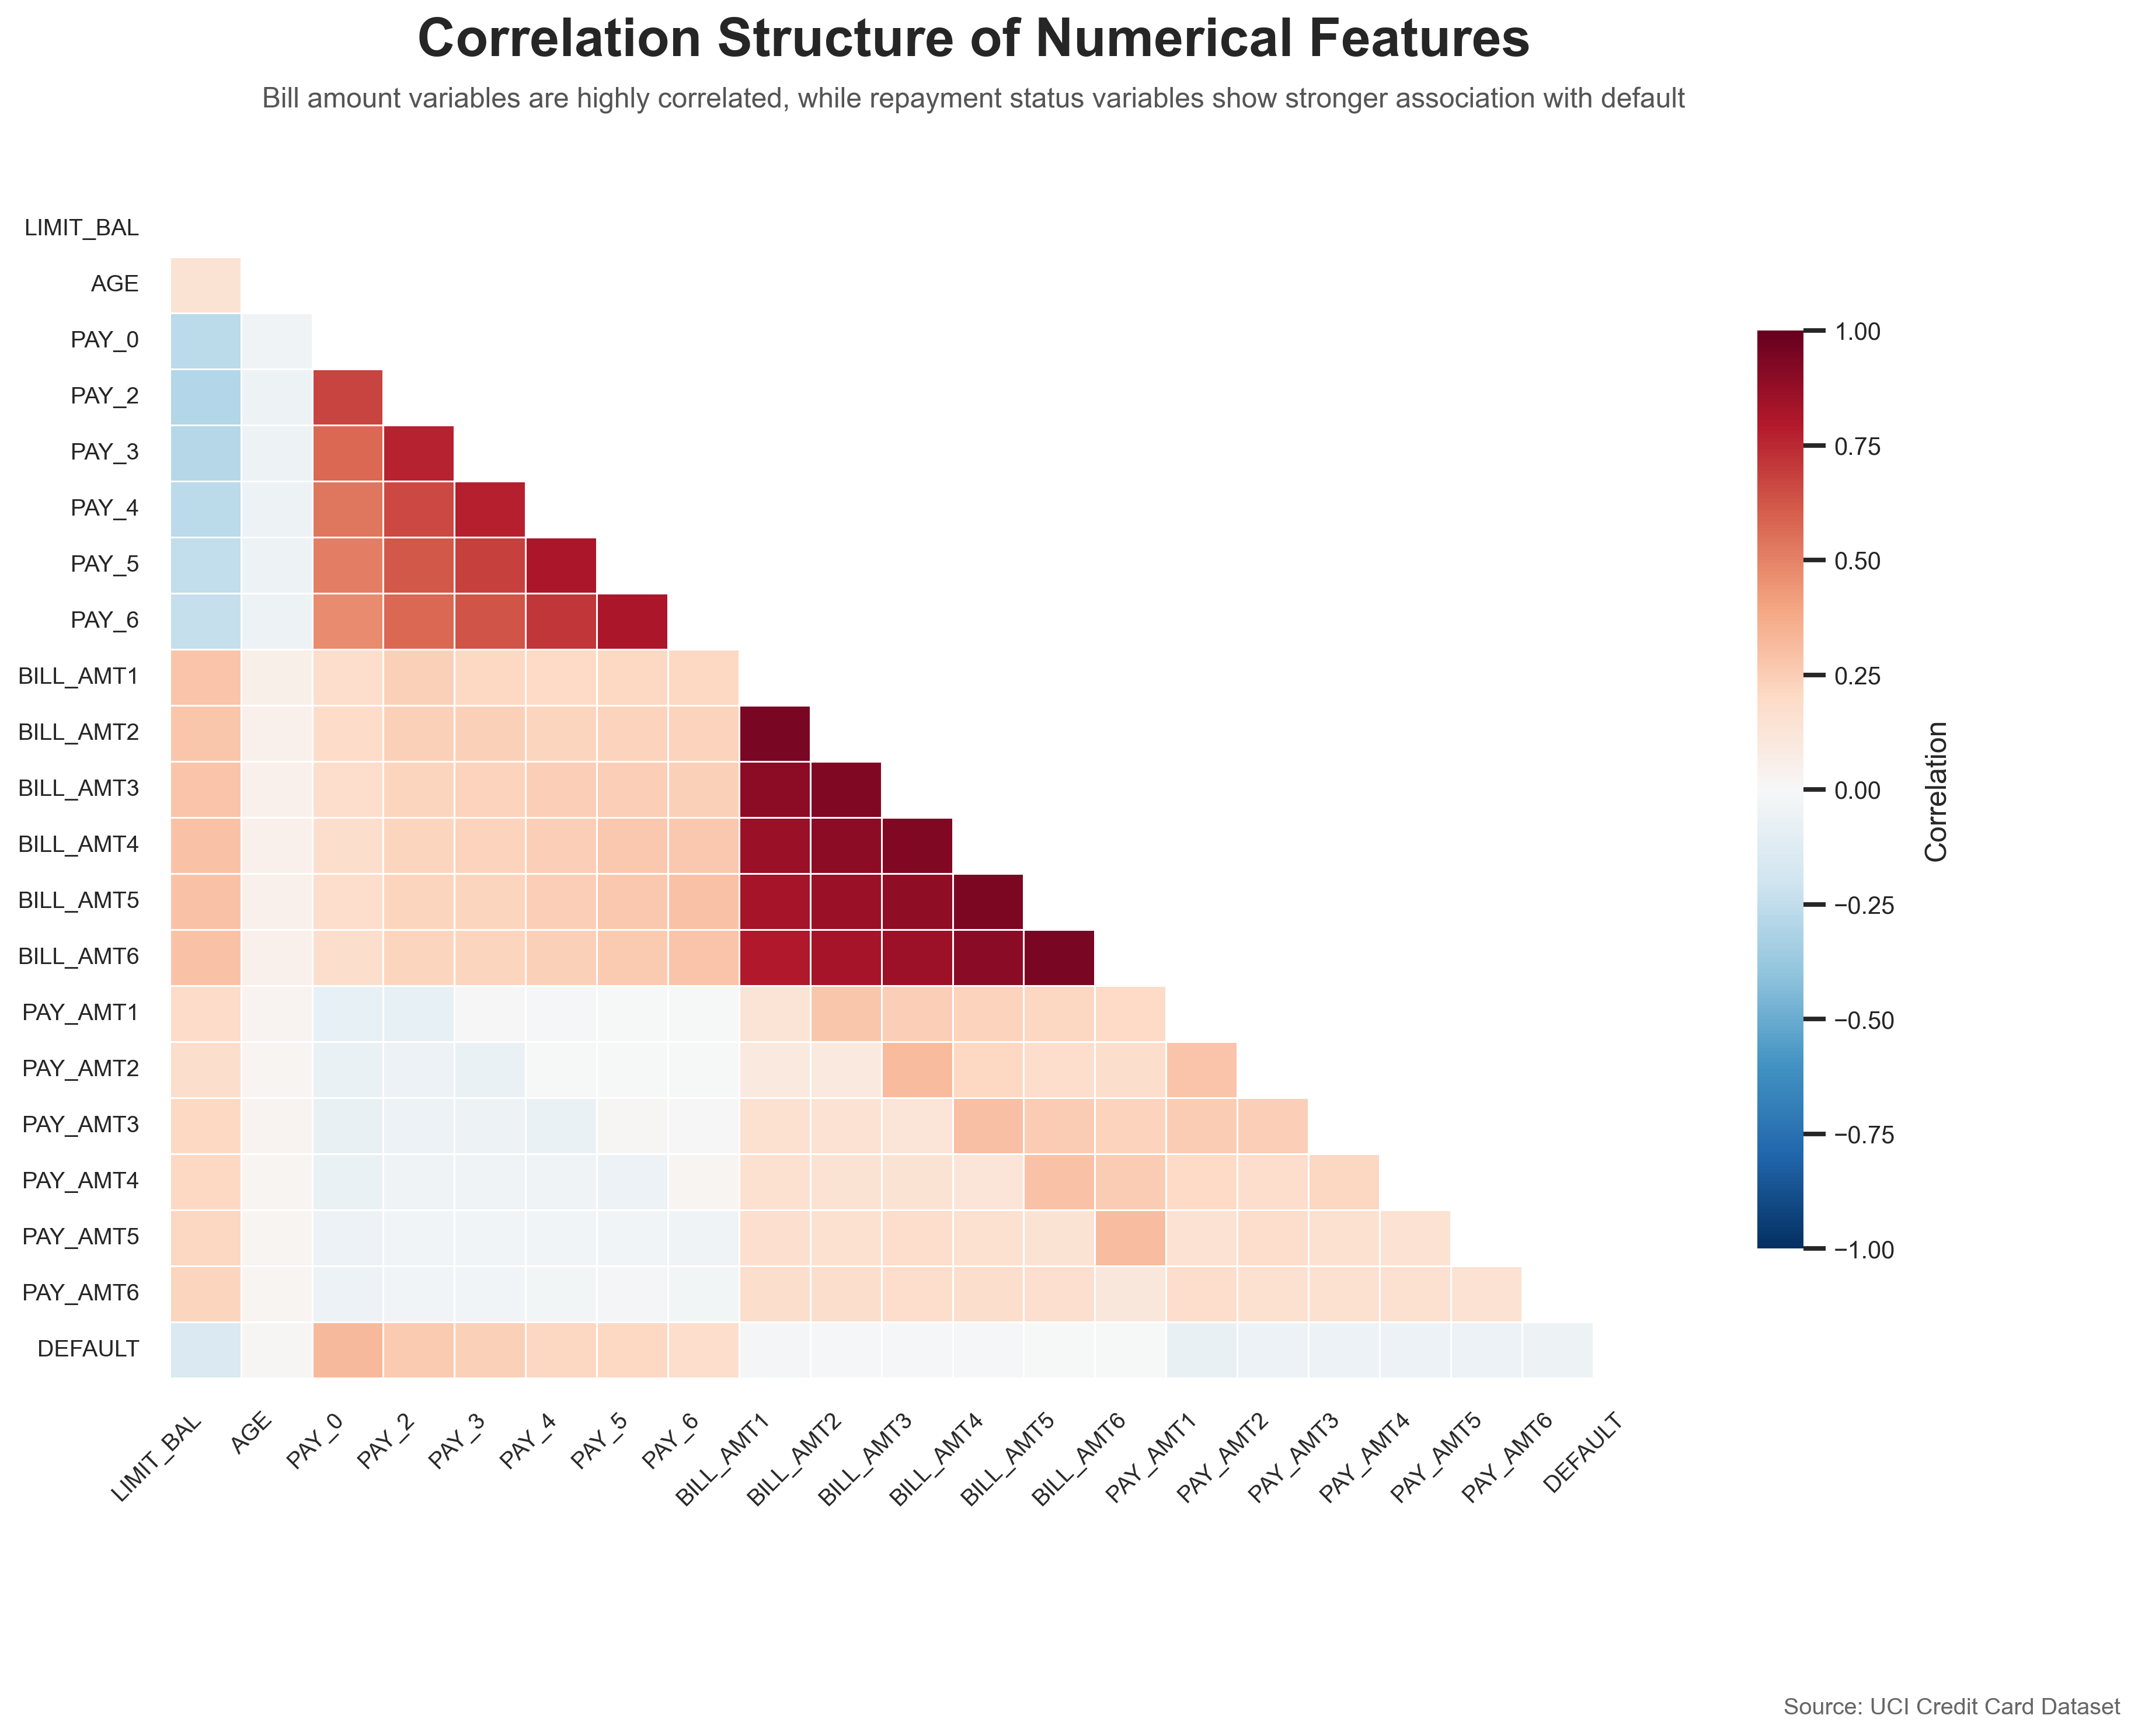
\includegraphics[width=0.48\textwidth]{09_feature_correlation_heatmap.png}
    \caption{Correlation heatmap of all features. Repayment status variables (PAY\_0 to PAY\_6) form a distinct cluster and show the highest correlation with the default target.}
    \label{fig:corr_heatmap}
\end{figure}

\begin{figure}[H]
    \centering
    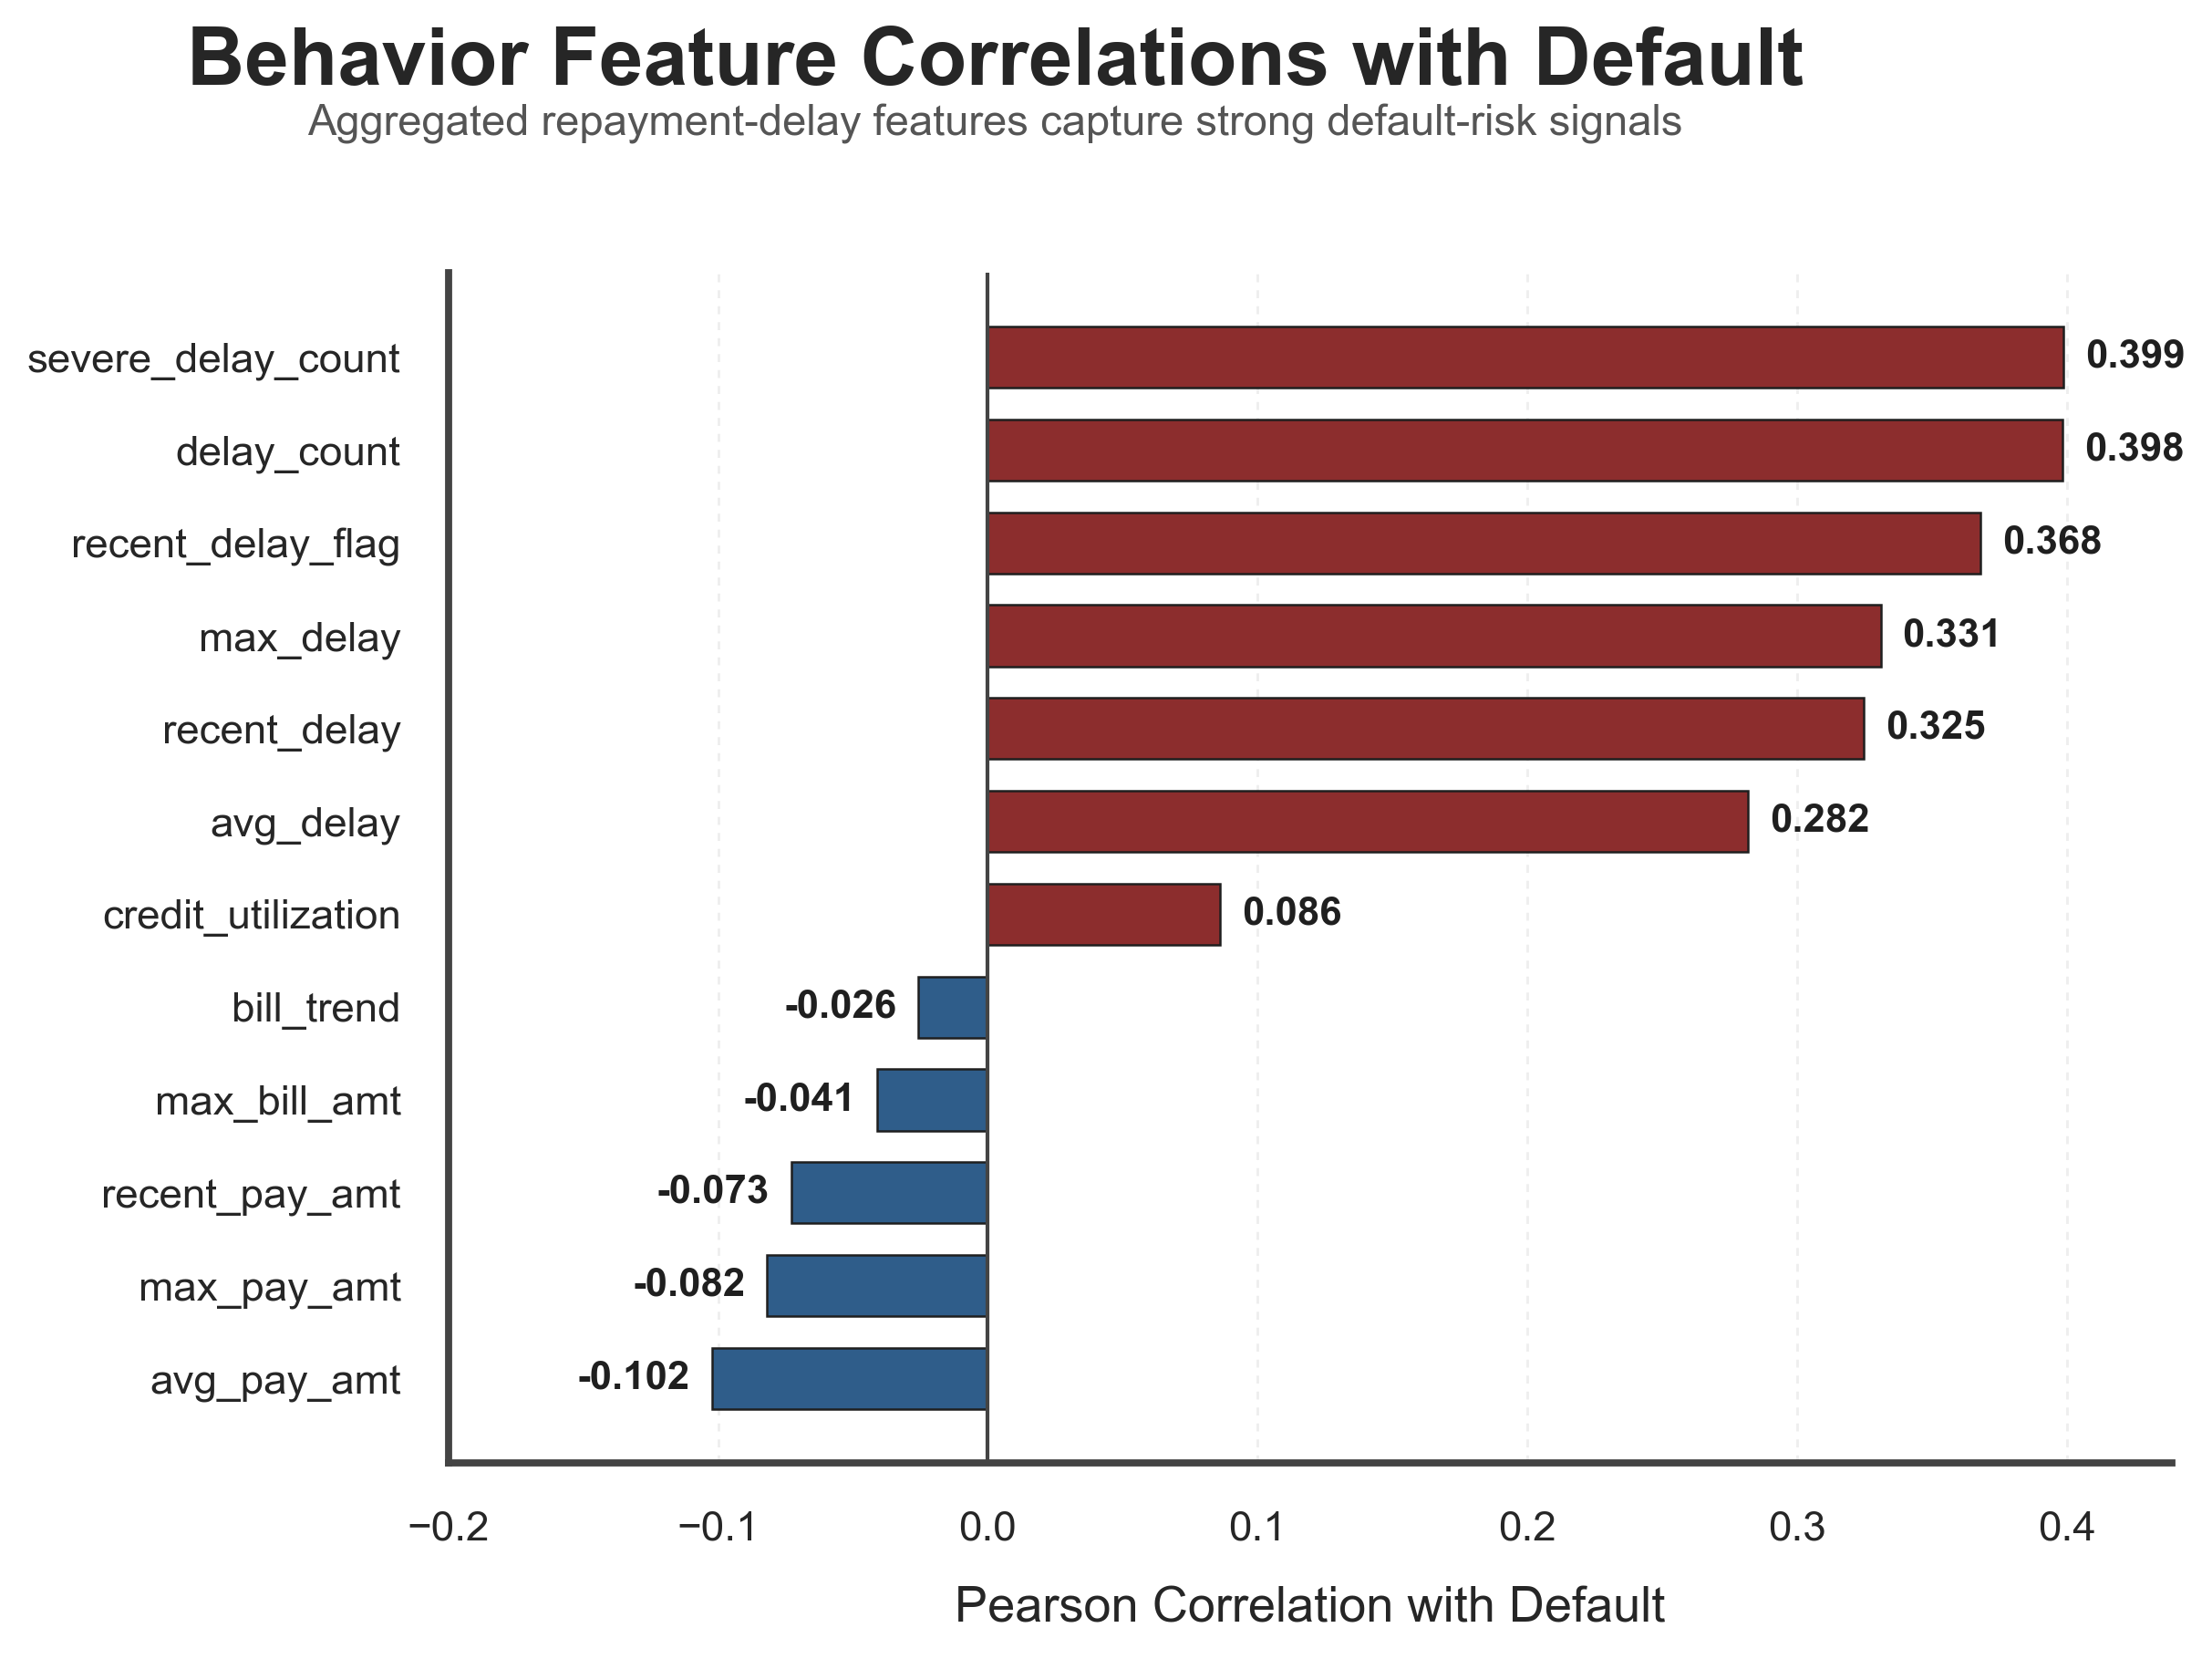
\includegraphics[width=0.48\textwidth]{10_behavior_feature_correlations_with_default.png}
    \caption{Correlation of engineered features with default. \emph{severe\_delay\_count} and \emph{delay\_count} exhibit the strongest association.}
    \label{fig:behavior_corr}
\end{figure}

PAY\_0 achieves a correlation coefficient of 0.325 with the target---substantially higher than any demographic or bill-amount variable. Our engineered features strengthen this signal further: \emph{severe\_delay\_count} (0.399) and \emph{delay\_count} (0.398) exceed any individual raw feature.

\subsection{Repayment Status and Default Risk}
The most recent repayment status exhibits a striking relationship with default probability. When PAY\_0 indicates no delay, the default rate is 13.8\% (baseline: 22.1\%). The rate increases sharply with delay severity: PAY\_0 = 2 reaches 69.1\%, and PAY\_0 = 3 reaches 75.8\%.

\begin{figure}[H]
    \centering
    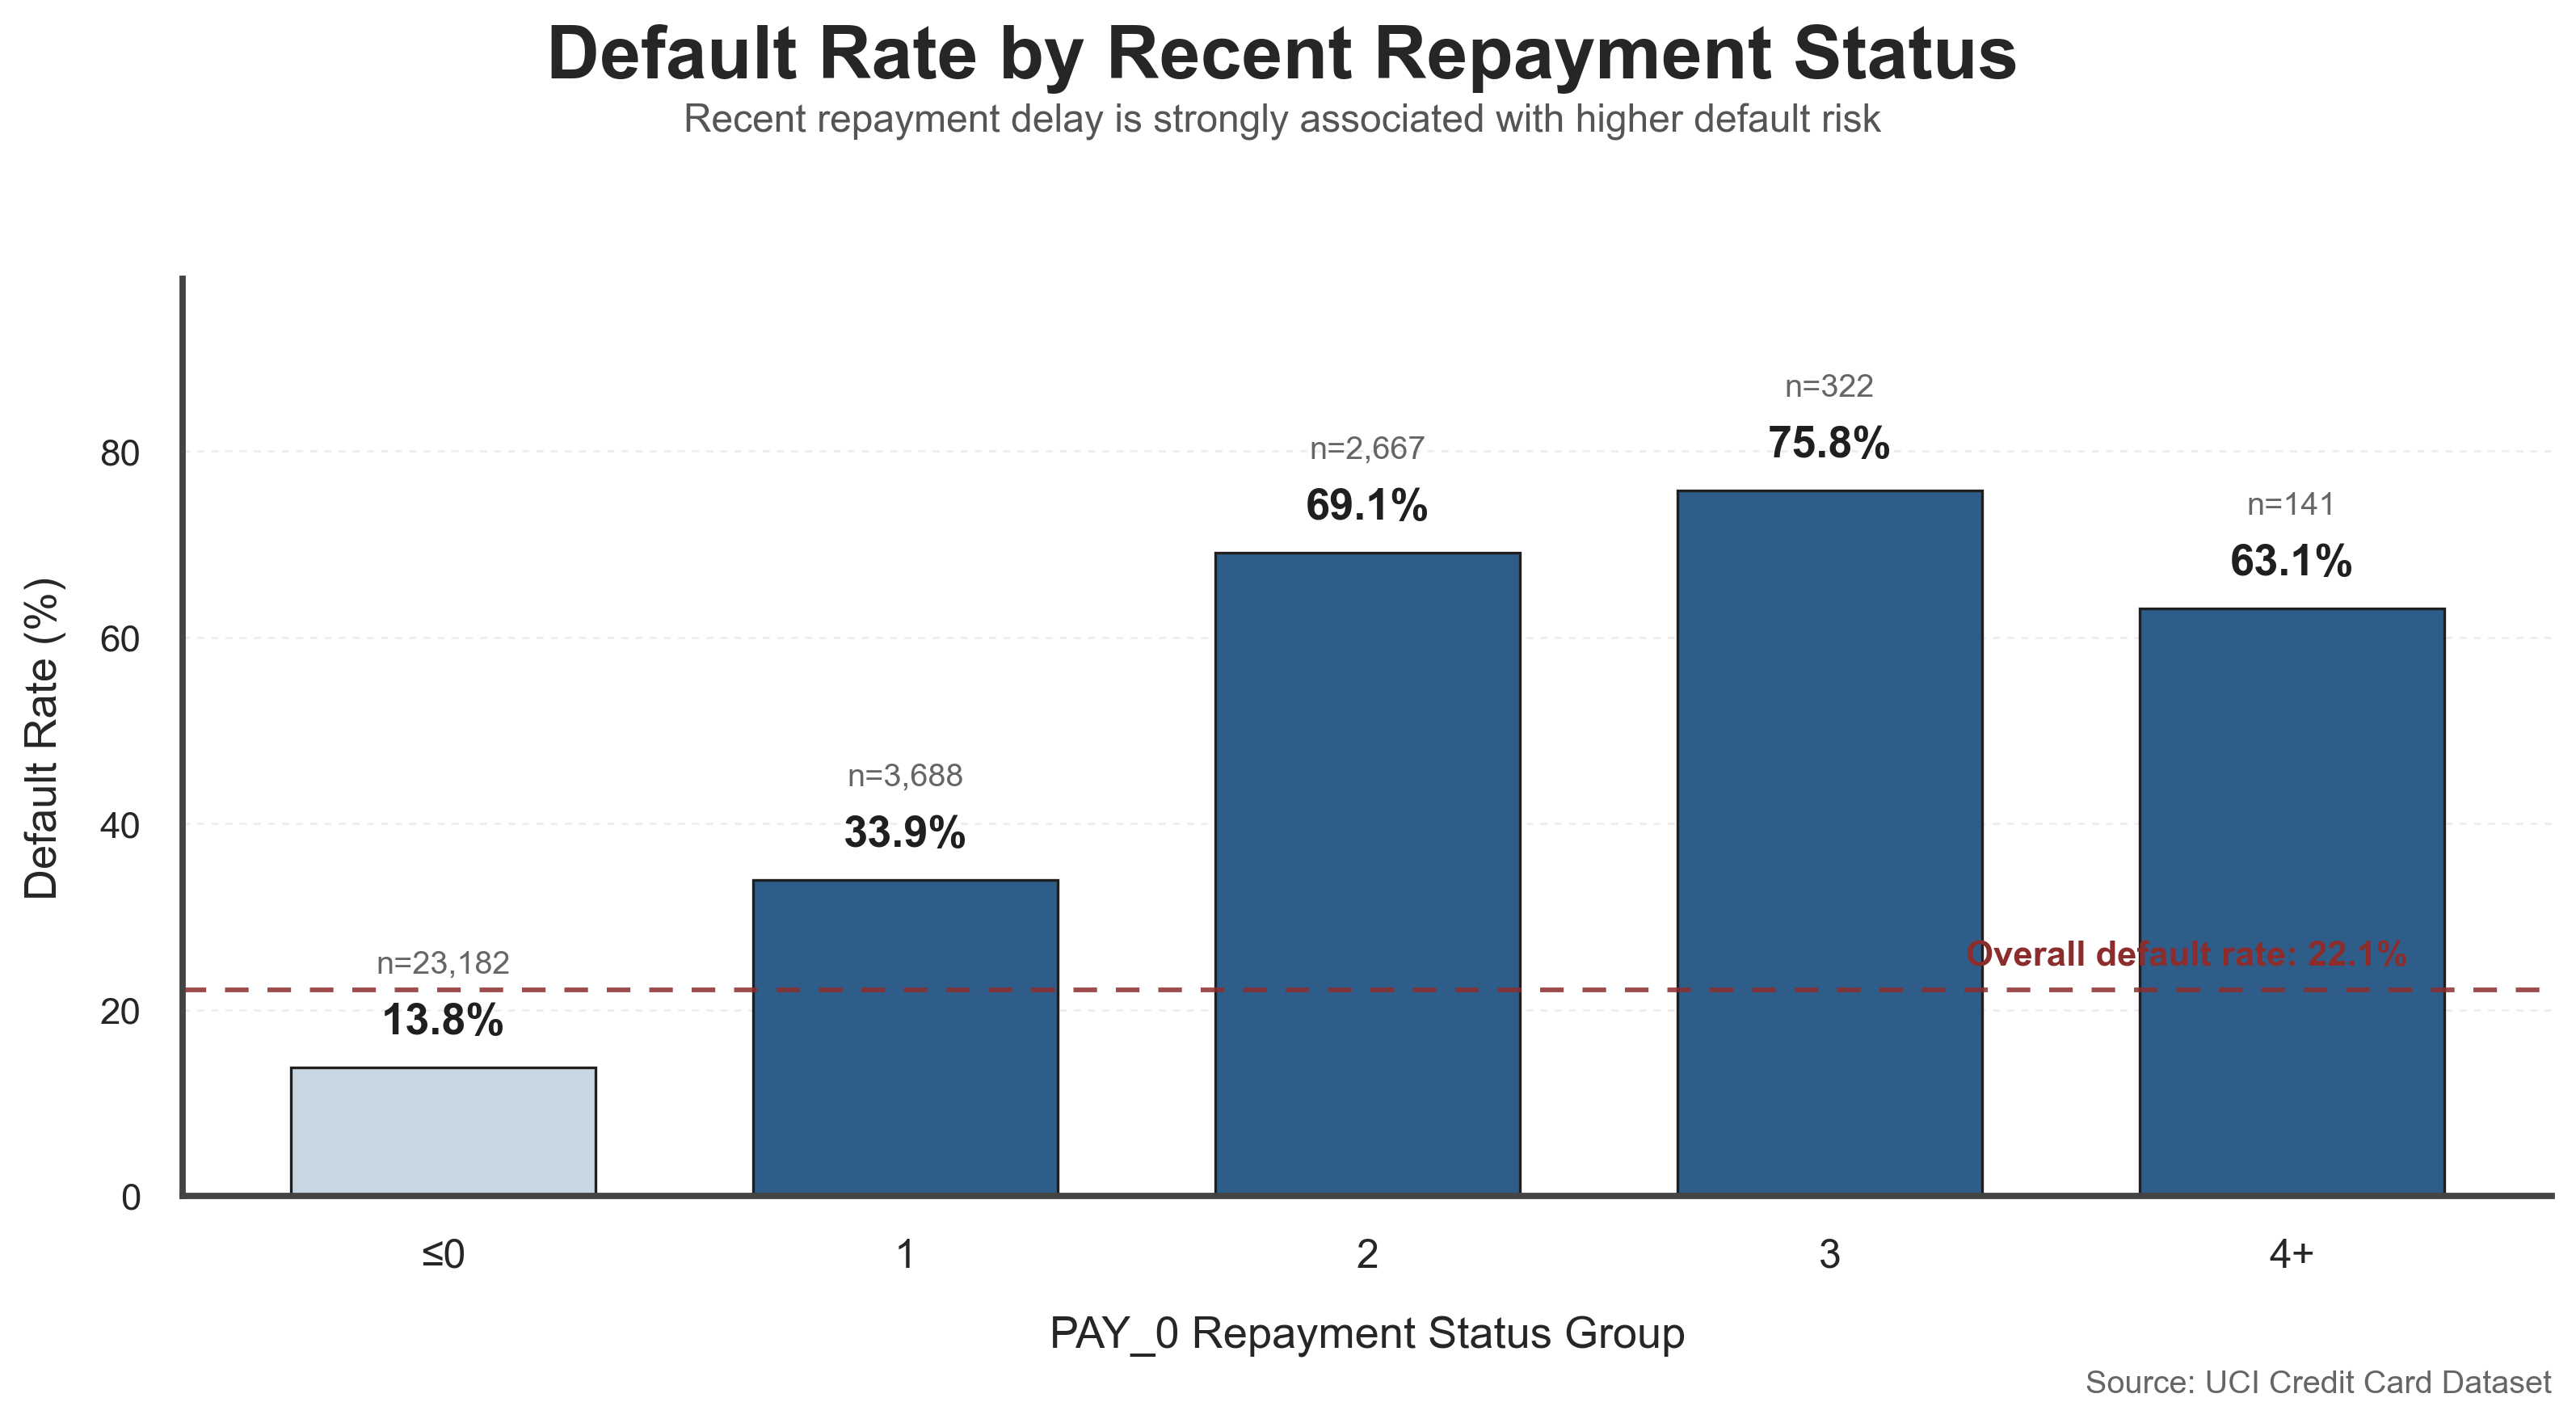
\includegraphics[width=0.48\textwidth]{05_default_rate_by_PAY_0_grouped_final.png}
    \caption{Default rate by grouped PAY\_0 status. A clear monotonic relationship is observed.}
    \label{fig:pay0_default}
\end{figure}

Figure~\ref{fig:delay_count} further confirms that historical delinquency frequency is a powerful risk indicator. Clients with zero past delinquencies default at 11.7\%, while those delinquent in all six months default at 70.3\%.

\begin{figure}[H]
    \centering
    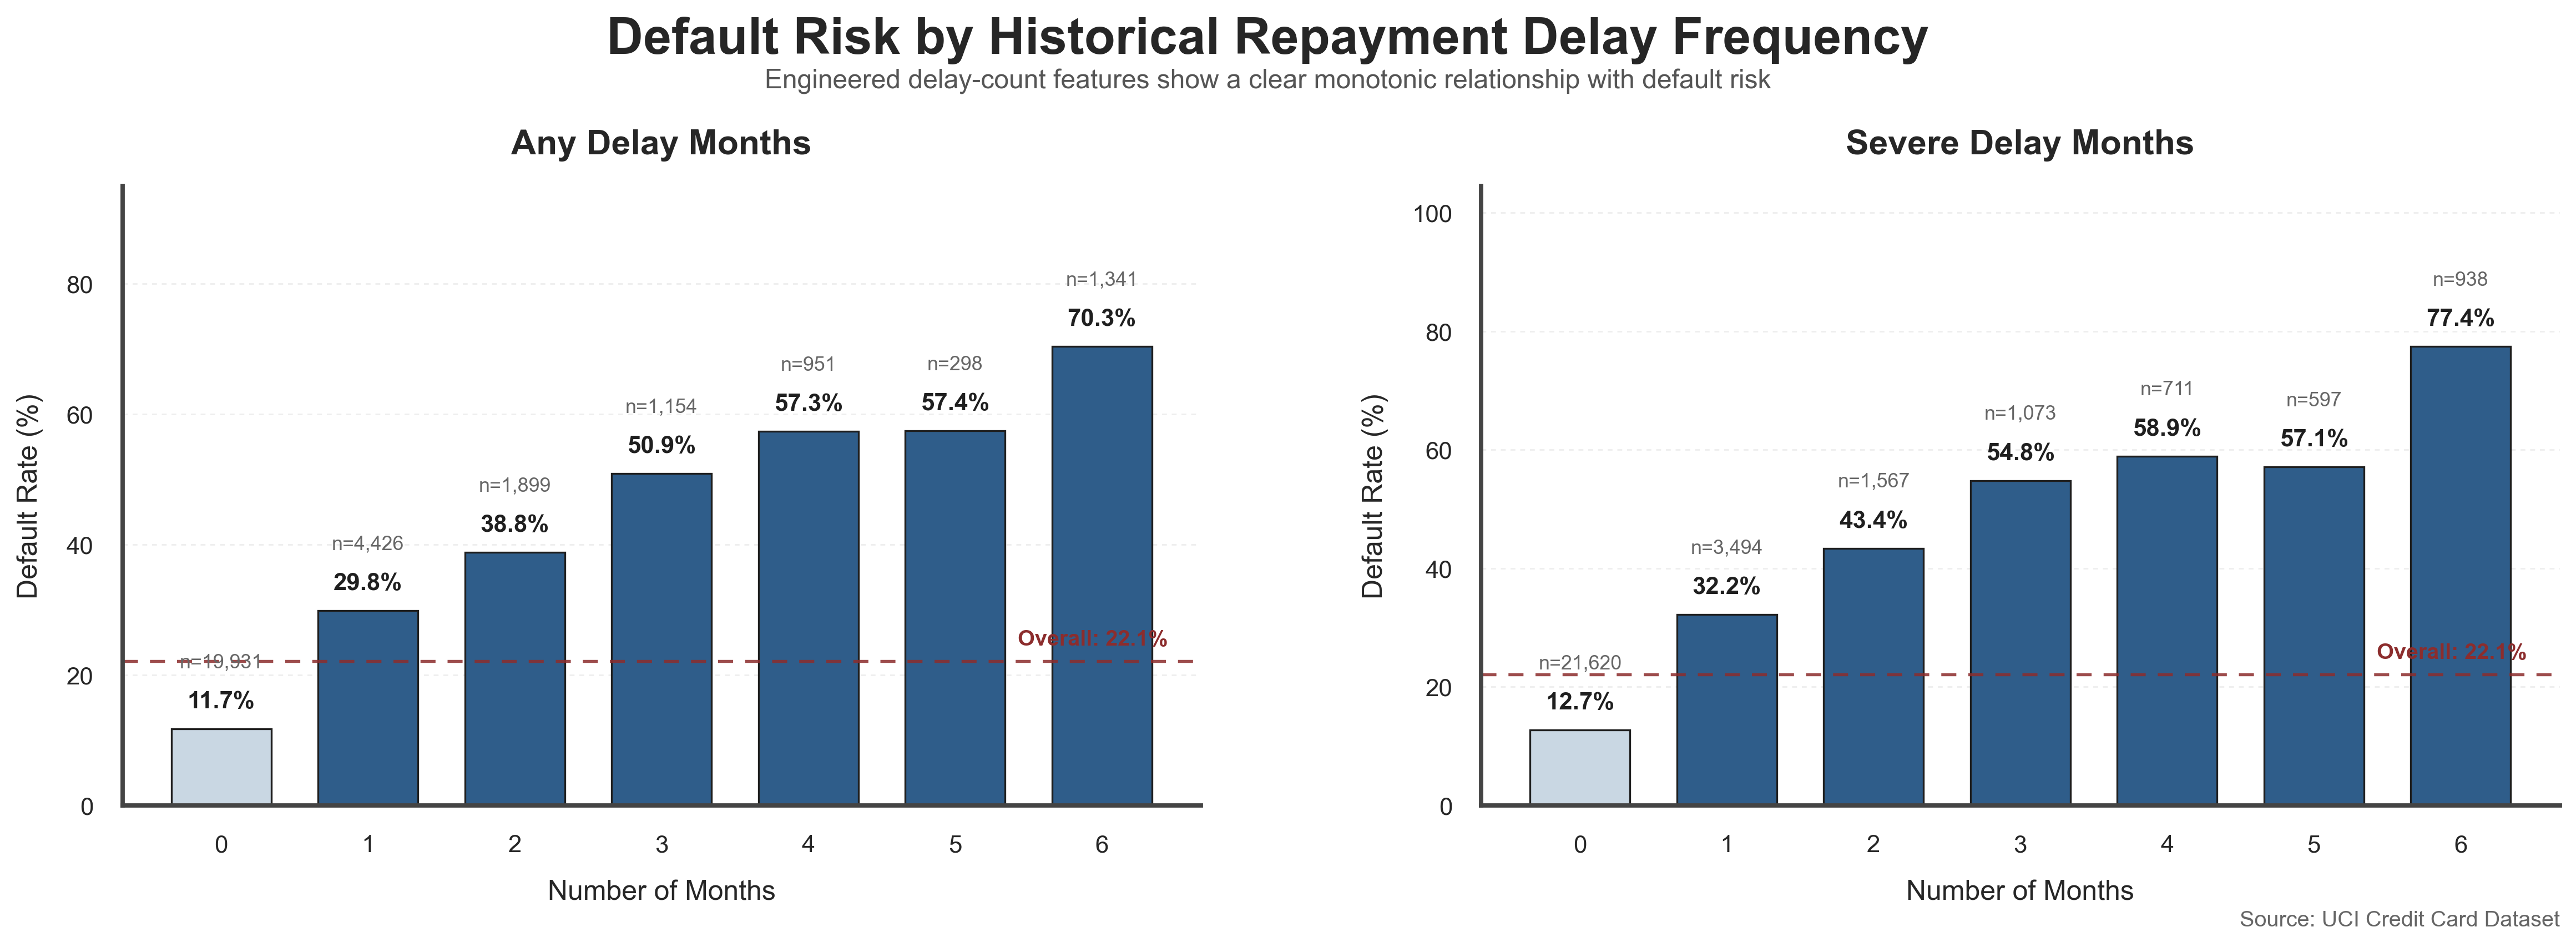
\includegraphics[width=0.48\textwidth]{11_default_rate_by_delay_count_features.png}
    \caption{Default rate by delinquency frequency. The monotonically increasing trend confirms that historical payment behavior is the most reliable indicator of future default.}
    \label{fig:delay_count}
\end{figure}

\section{Methodology}

\subsection{Data Preprocessing}
We applied three preprocessing steps. First, non-standard categorical encodings were fixed: EDUCATION values of 0, 5, and 6 were mapped to category 4, and MARRIAGE value 0 was mapped to 3. Second, a stratified 80/20 train-test split preserved the class distribution. Third, StandardScaler normalization was applied to ensure zero mean and unit variance.

\subsection{Feature Engineering}
Building on the EDA findings, we constructed 17 repayment-behavior features that summarize clients' historical payment patterns. They fall into four groups:

\textbf{Delay behavior:} \emph{delay\_count} (number of months delayed), \emph{severe\_delay\_count} ($\geq$~2 months), \emph{max\_delay}, \emph{avg\_delay}, \emph{recent\_delay\_flag}.

\textbf{Bill behavior:} \emph{avg\_bill\_amt}, \emph{max\_bill\_amt}, \emph{bill\_trend}, \emph{credit\_utilization} (bill/limit).

\textbf{Payment behavior:} \emph{avg\_pay\_amt}, \emph{max\_pay\_amt}, \emph{pay\_trend}.

\textbf{Ratios:} \emph{recent\_pay\_bill\_ratio}, \emph{total\_pay\_bill\_ratio}.

This yields two feature sets: Set A (23 raw features) and Set B (40 features = 23 raw + 17 engineered).

\subsection{Machine Learning Models}
We evaluated seven classifiers: Logistic Regression (balanced class weights, L2 regularization), Decision Tree ($\text{max\_depth}=8$, balanced), KNN ($k=5$), Linear SVM with probability calibration, Random Forest (200 trees, $\text{max\_depth}=12$), Gradient Boosting, and XGBoost~\cite{chen2016xgboost}.

\subsection{Deep Neural Network}
We implemented a DNN in PyTorch. The baseline has three hidden layers (128, 64, 32) with BatchNorm, ReLU, and dropout (0.3). The optimized variant uses four layers (256, 128, 64, 32), LeakyReLU, Kaiming initialization, ReduceLROnPlateau scheduling, and gradient clipping at norm~1.0.

To address class imbalance, we compared:

\textbf{Binary Cross-Entropy:}
\begin{equation}
    \mathcal{L}_{\text{BCE}} = -\frac{1}{N}\sum_{i=1}^{N}[y_i\log(\hat{y}_i) + (1-y_i)\log(1-\hat{y}_i)]
\end{equation}

\textbf{Weighted BCE:} where $w_p$ weights the positive class:
\begin{equation}
    \mathcal{L}_{\text{WBCE}} = -\frac{1}{N}\sum_{i=1}^{N}[w_p\, y_i\log(\hat{y}_i) + (1-y_i)\log(1-\hat{y}_i)]
\end{equation}
Our best configuration uses $w_p = 2.0$.

\textbf{Focal Loss~\cite{lin2017focal}:}
\begin{equation}
    \mathcal{L}_{\text{focal}} = -\frac{1}{N}\sum_{i=1}^{N}\alpha(1-p_t)^\gamma\log(p_t)
\end{equation}
where $p_t = \hat{y}_i$ when $y_i=1$ and $p_t = 1-\hat{y}_i$ when $y_i=0$, with $\alpha=0.75,\;\gamma=2.0$.

\section{Experimental Results}

\subsection{Evaluation Metrics}
Given the moderate class imbalance and the risk-sensitive nature of credit default prediction, relying solely on accuracy is misleading. We prioritize recall (sensitivity), as failing to identify a defaulting client incurs severe financial losses. Precision is evaluated to measure operational efficiency, ensuring that collection resources are not wasted on false alarms. As our primary aggregate metrics, we report the F1-score and the area under the precision-recall curve (PR-AUC), which provide a more robust assessment under class imbalance. Finally, the ROC-AUC is utilized to measure the overall discriminatory power of the classifiers across all possible decision thresholds.

\subsection{Model Comparison}
Table~\ref{tab:model_ranking} presents the performance comparison on feature Set B.

\begin{table}[H]
    \centering
    \caption{Model Performance on Set B (Ranked by F1-score)}
    \label{tab:model_ranking}
    \footnotesize
    \renewcommand{\tabcolsep}{2.5pt}
    \begin{tabular}{lrrrrrr}
        \toprule
        Model & Acc. & Prec. & Rec. & F1 & AUC & PR \\
        \midrule
        Random Forest & 0.792 & 0.529 & 0.558 & 0.543 & 0.779 & 0.555 \\
        XGBoost & 0.767 & 0.479 & 0.605 & 0.534 & 0.772 & 0.547 \\
        Decision Tree & 0.732 & 0.431 & 0.662 & 0.522 & 0.765 & 0.529 \\
        Logistic Regression & 0.756 & 0.460 & 0.597 & 0.520 & 0.758 & 0.524 \\
        Gradient Boosting & 0.818 & 0.659 & 0.366 & 0.471 & 0.778 & 0.551 \\
        SVM & 0.816 & 0.656 & 0.354 & 0.460 & 0.756 & 0.517 \\
        KNN & 0.793 & 0.547 & 0.366 & 0.439 & 0.708 & 0.422 \\
        \bottomrule
    \end{tabular}
\end{table}

Random Forest achieves the highest F1-score (0.543) and ROC-AUC (0.779). XGBoost achieves the best recall (0.605). Gradient Boosting and SVM attain high accuracy and precision but suffer from low recall, indicating they are overly conservative in predicting defaults.

\begin{figure}[H]
    \centering
    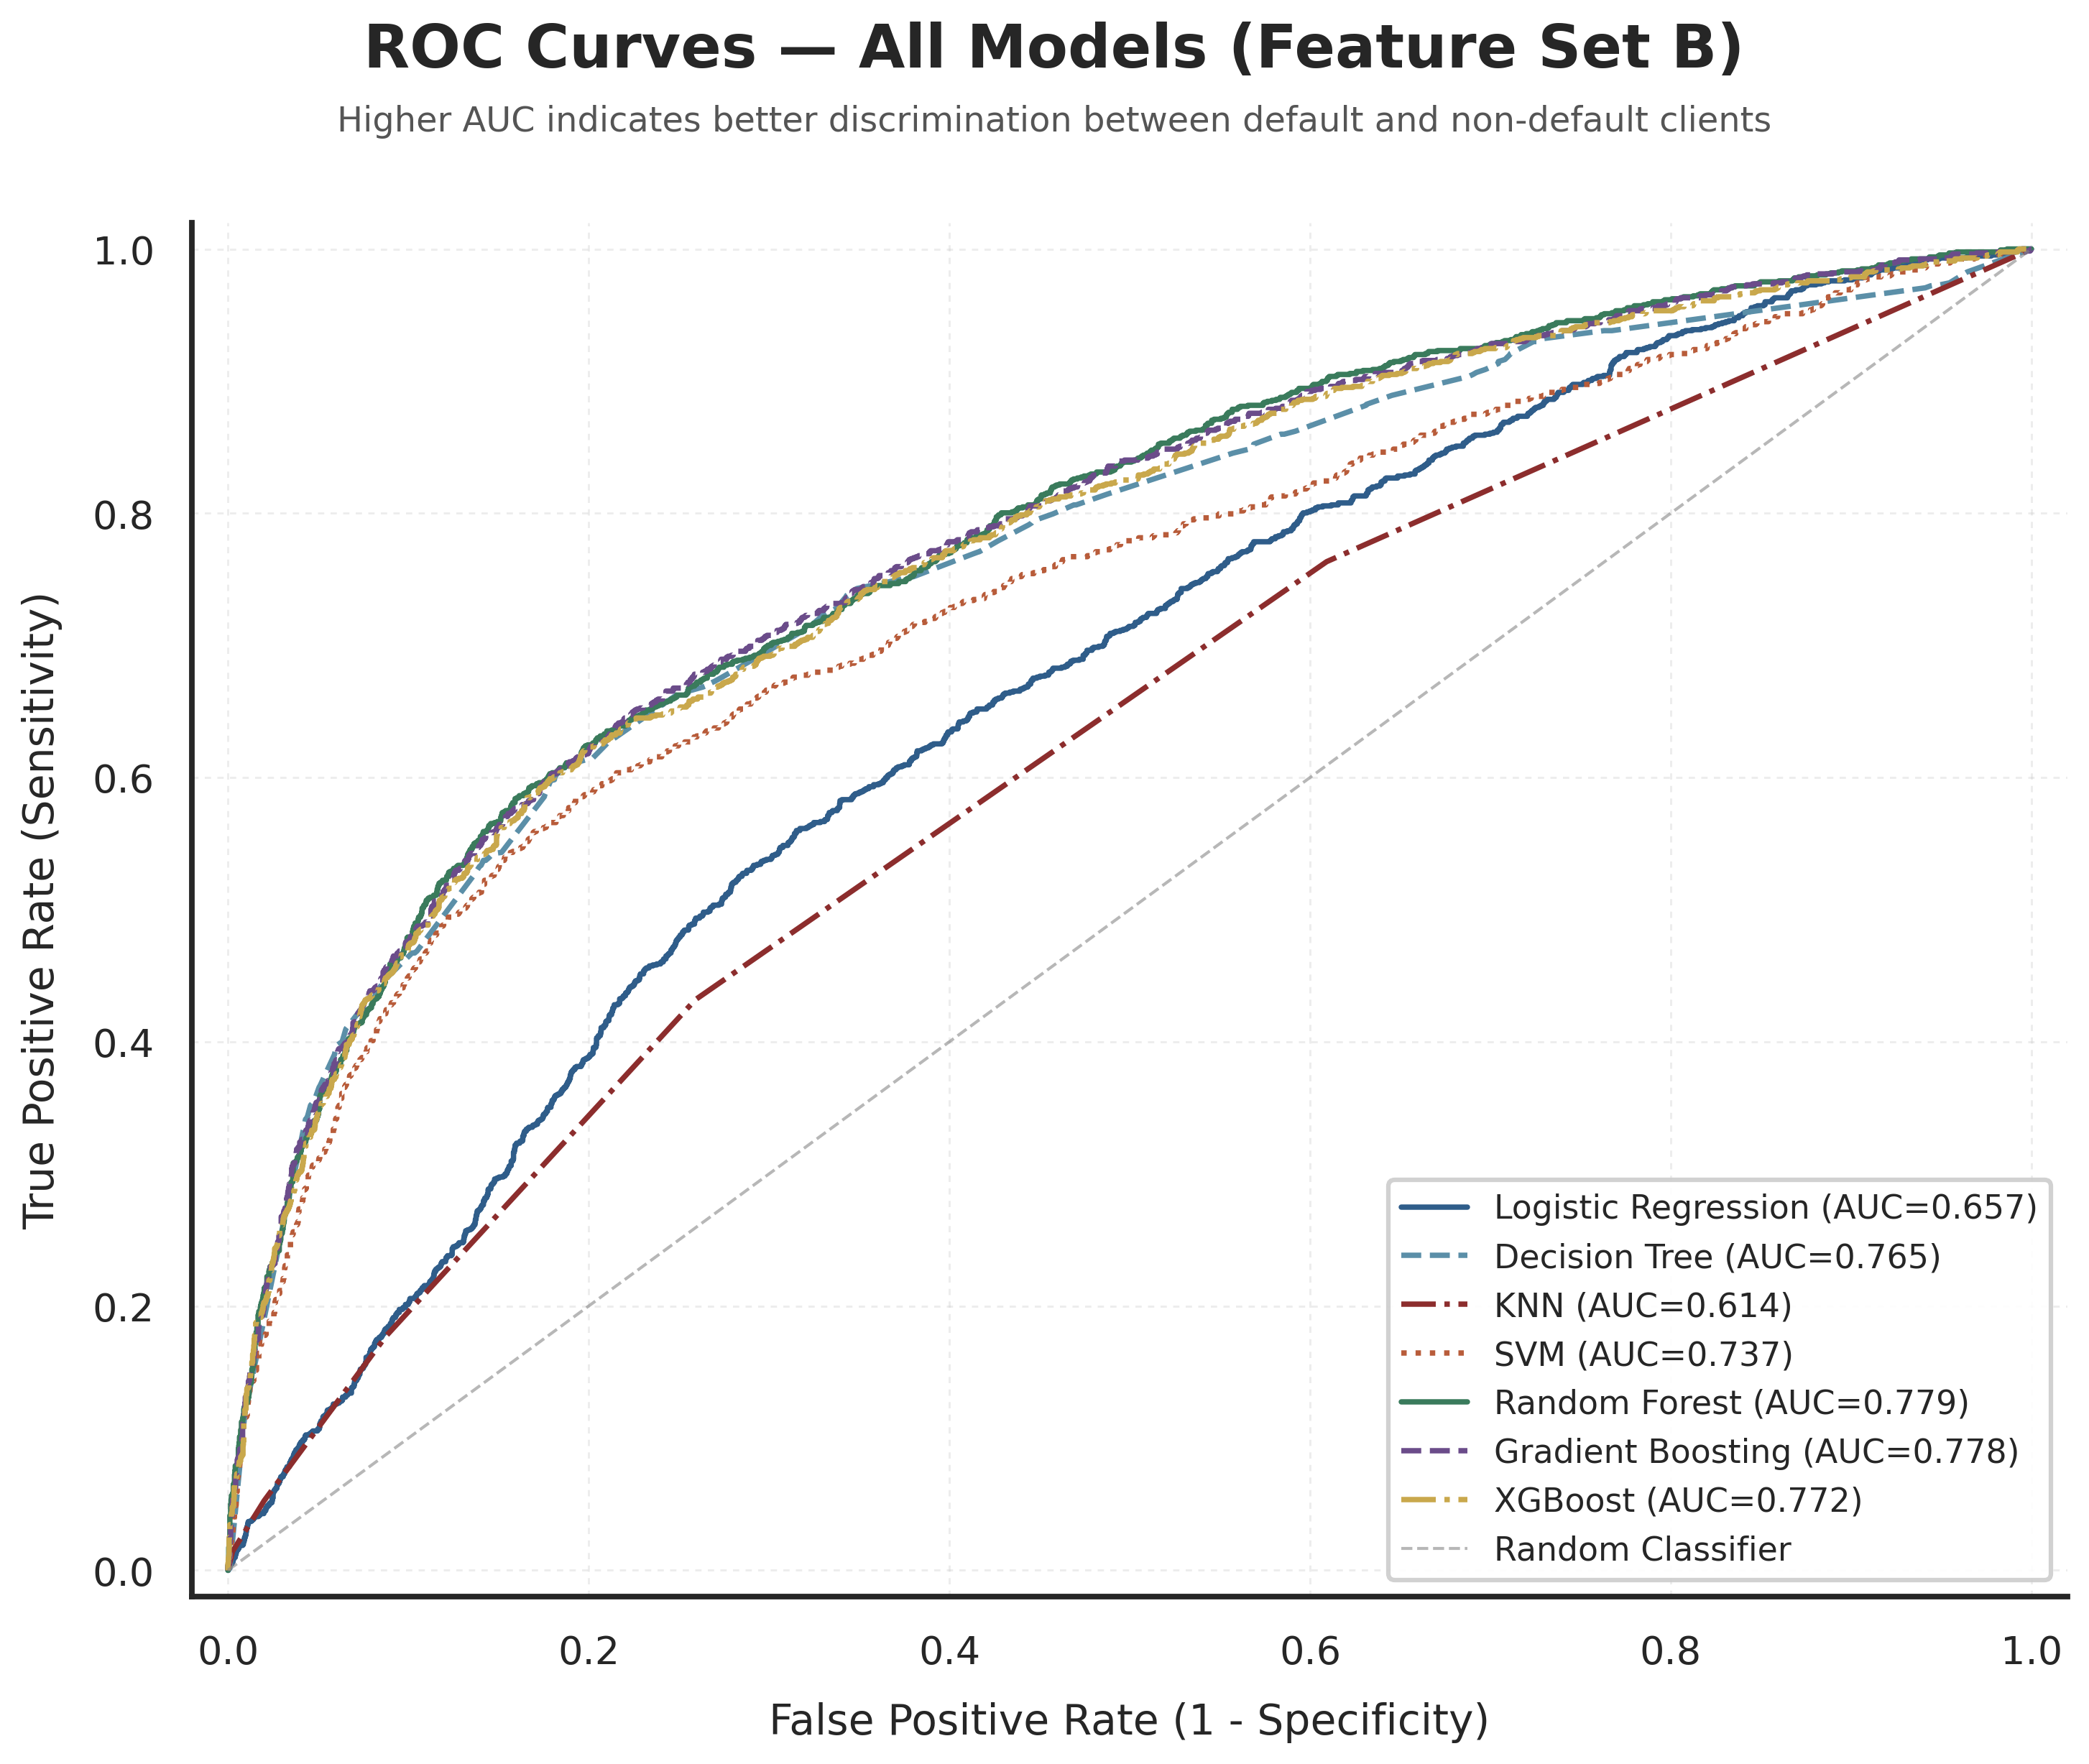
\includegraphics[width=0.48\textwidth]{19_roc_curves_all_models.png}
    \caption{ROC curves for all models. Random Forest and XGBoost show the best trade-off.}
    \label{fig:roc}
\end{figure}

\subsection{Feature Set Comparison}
Table~\ref{tab:feature_set} compares performance with and without engineered features.

\begin{table}[H]
    \centering
    \caption{F1 Improvement with Engineered Features}
    \label{tab:feature_set}
    \footnotesize
    \renewcommand{\tabcolsep}{4pt}
    \begin{tabular}{lrrr}
        \toprule
        Model & F1 (A) & F1 (B) & $\Delta$F1 \\
        \midrule
        Logistic Regression & 0.461 & 0.520 & +0.059 \\
        Decision Tree & 0.508 & 0.522 & +0.014 \\
        KNN & 0.429 & 0.439 & +0.010 \\
        SVM & 0.356 & 0.460 & +0.104 \\
        Random Forest & 0.543 & 0.543 & 0.000 \\
        Gradient Boosting & 0.462 & 0.471 & +0.009 \\
        XGBoost & 0.522 & 0.534 & +0.012 \\
        \bottomrule
    \end{tabular}
\end{table}

The engineered features provide the most dramatic improvement for simpler models: Logistic Regression's F1 improves by 5.9~pp, and SVM improves by 10.4~pp. For ensemble methods, the gain is more modest, suggesting they already extract useful patterns from raw features.

\subsection{DNN Training Dynamics}
Figure~\ref{fig:dnn_learning} shows the learning curves of the baseline DNN, illustrating training and validation loss together with validation AUC across 31 epochs before early stopping.

\begin{figure}[H]
    \centering
    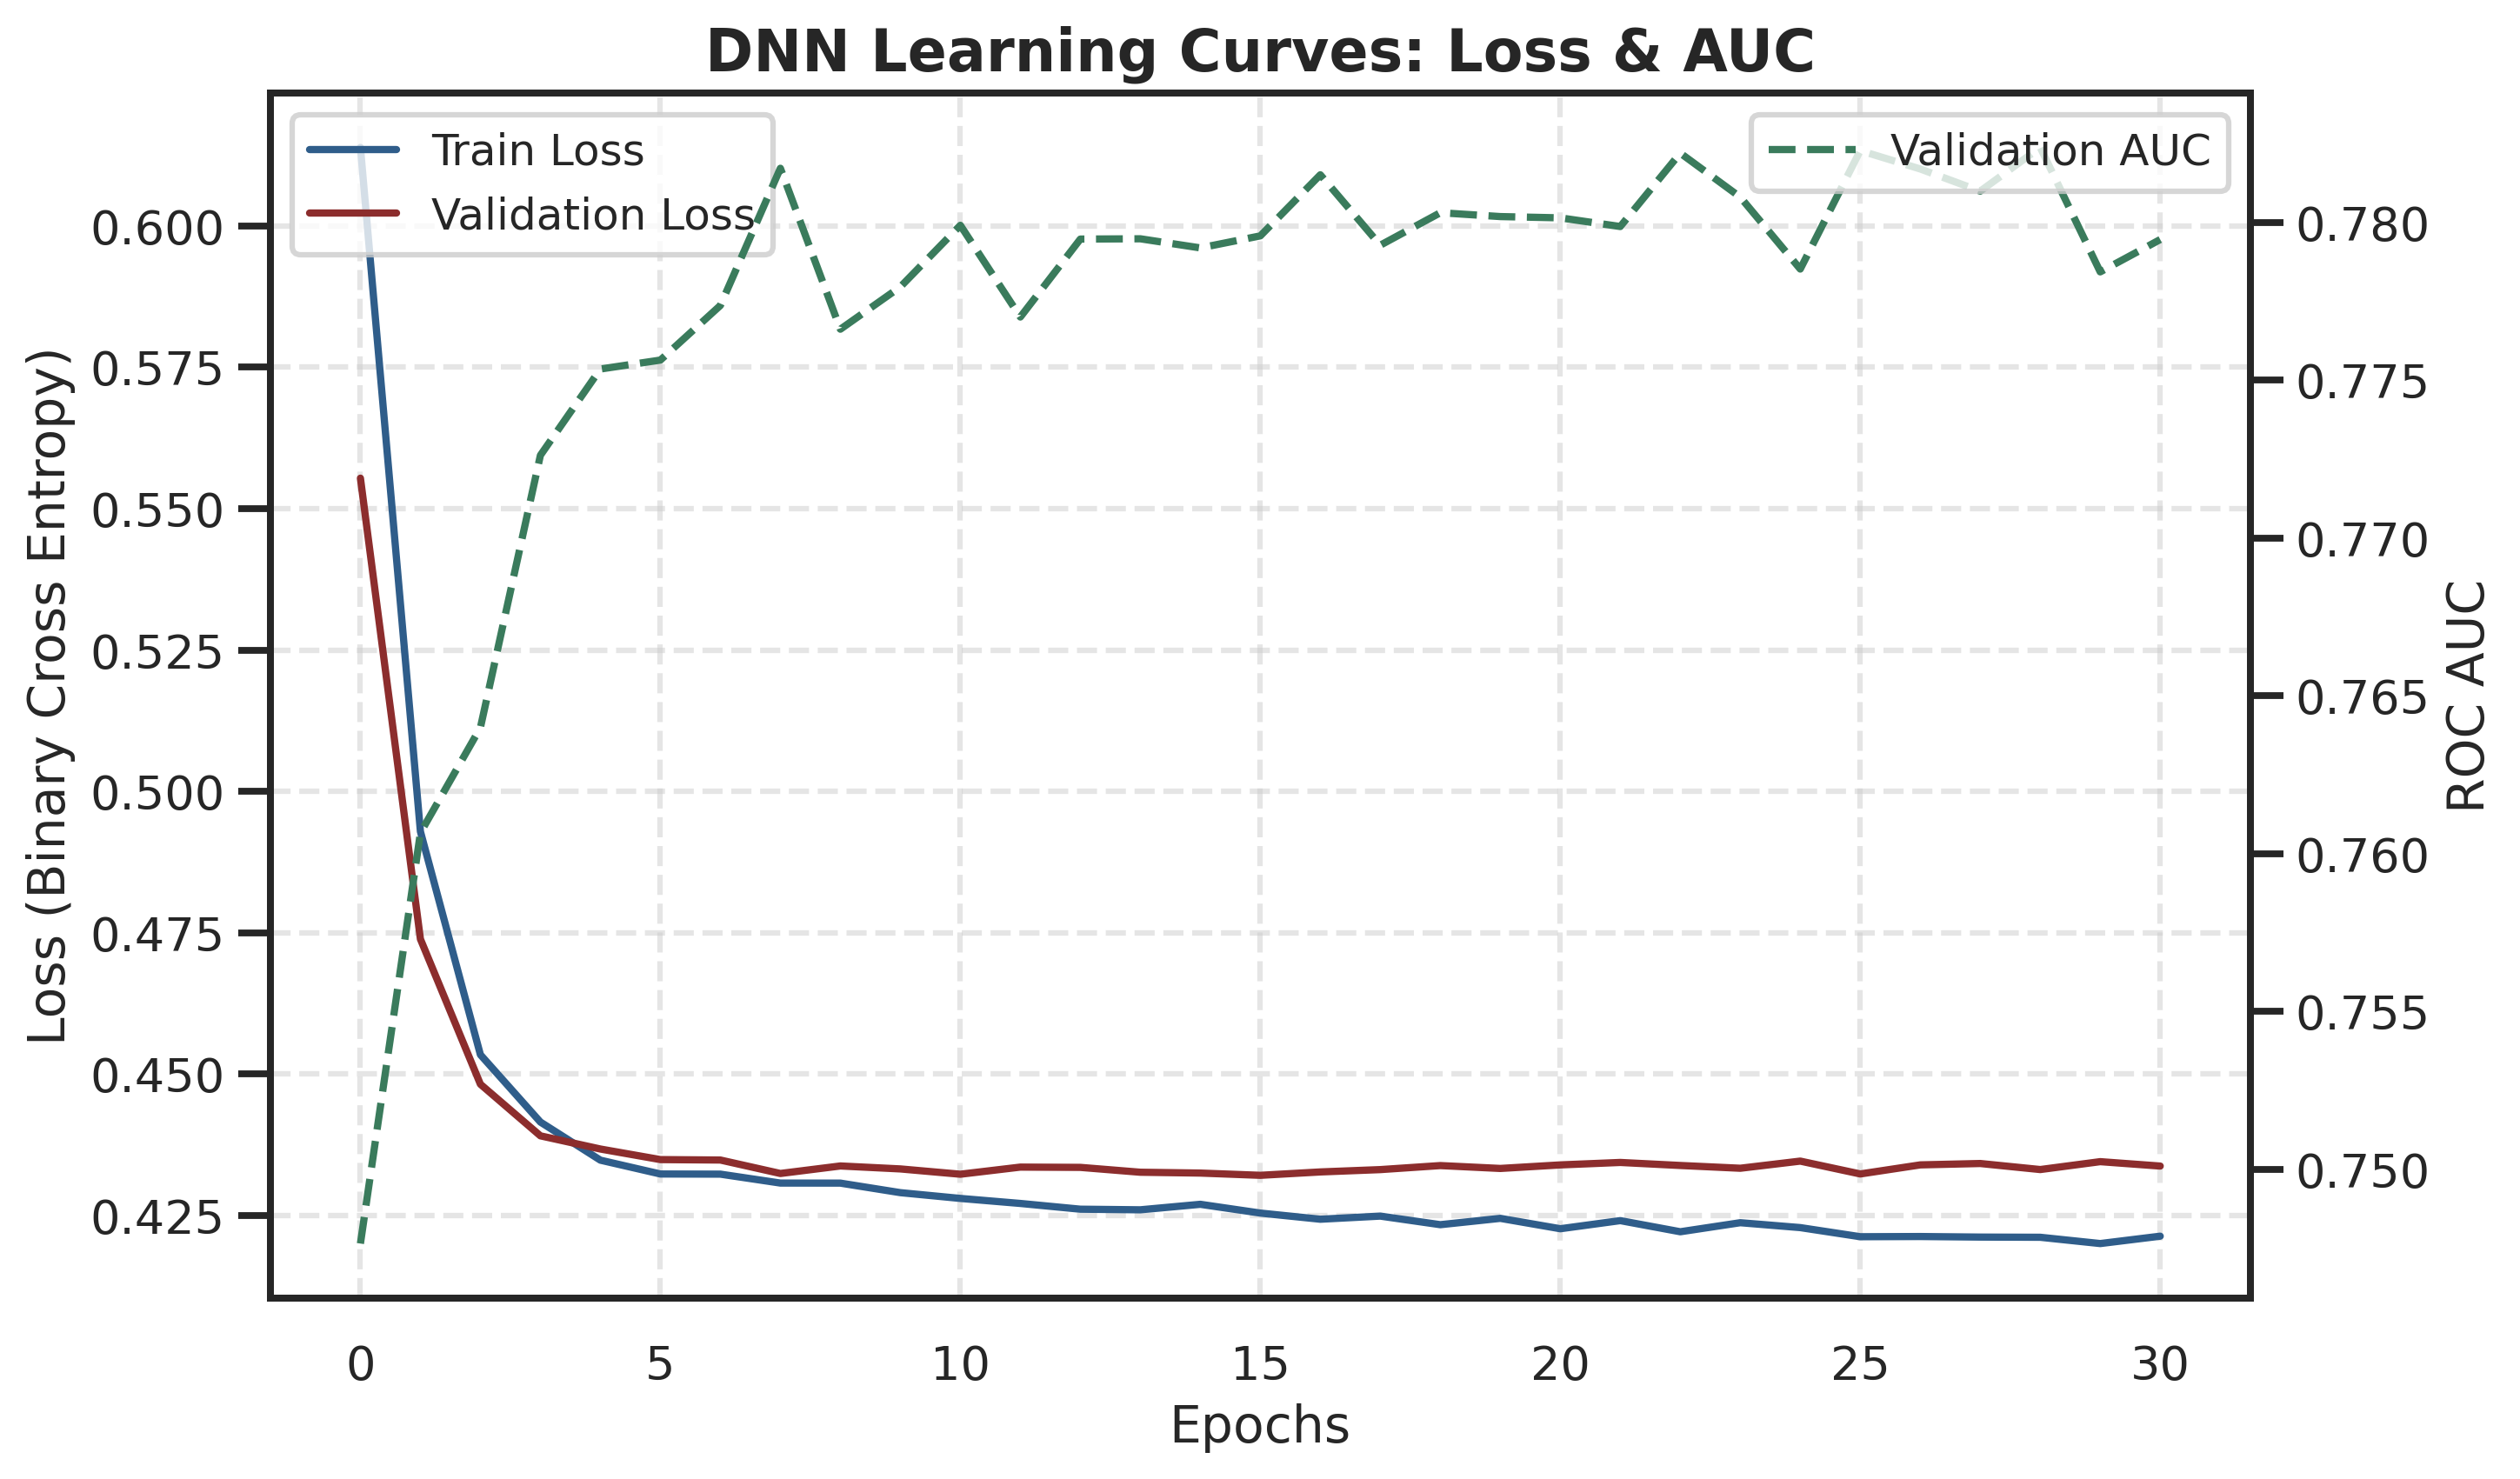
\includegraphics[width=0.48\textwidth]{29_dnn_learning_curves.png}
    \caption{DNN learning curves. Early stopping at epoch~31 prevents overfitting.}
    \label{fig:dnn_learning}
\end{figure}

\subsection{DNN Optimization Results}
The baseline DNN with standard BCE achieves an F1 of 0.477. The choice of loss function proves critical. Table~\ref{tab:dnn_opt} presents the optimization results.

\begin{table}[H]
    \centering
    \caption{DNN Optimization Across Loss Functions}
    \label{tab:dnn_opt}
    \footnotesize
    \renewcommand{\tabcolsep}{3pt}
    \begin{tabular}{lrrrrr}
        \toprule
        Variant & Acc. & Prec. & Rec. & F1 & AUC \\
        \midrule
        Baseline BCE & 0.819 & 0.661 & 0.373 & 0.477 & 0.774 \\
        BCE + Scheduler & 0.816 & 0.649 & 0.365 & 0.467 & 0.775 \\
        \textbf{Weighted BCE (2.0)} & \textbf{0.805} & \textbf{0.565} & \textbf{0.509} & \textbf{0.536} & \textbf{0.777} \\
        Focal Loss & 0.780 & 0.502 & 0.564 & 0.531 & 0.774 \\
        Ensemble (5 seeds) & 0.787 & 0.516 & 0.553 & 0.534 & 0.775 \\
        \bottomrule
    \end{tabular}
\end{table}

Weighted BCE ($w_p=2.0$) achieves the highest F1 (0.536), improving the baseline by 5.9~pp. This comes at the cost of reduced precision (0.565 vs.~0.661) but substantially improved recall (0.509 vs.~0.373). Focal Loss achieves the best recall among DNN variants (0.564). These results demonstrate that simple loss-function modification yields DNN performance comparable to sophisticated ensemble methods without architectural changes.

\begin{figure}[H]
    \centering
    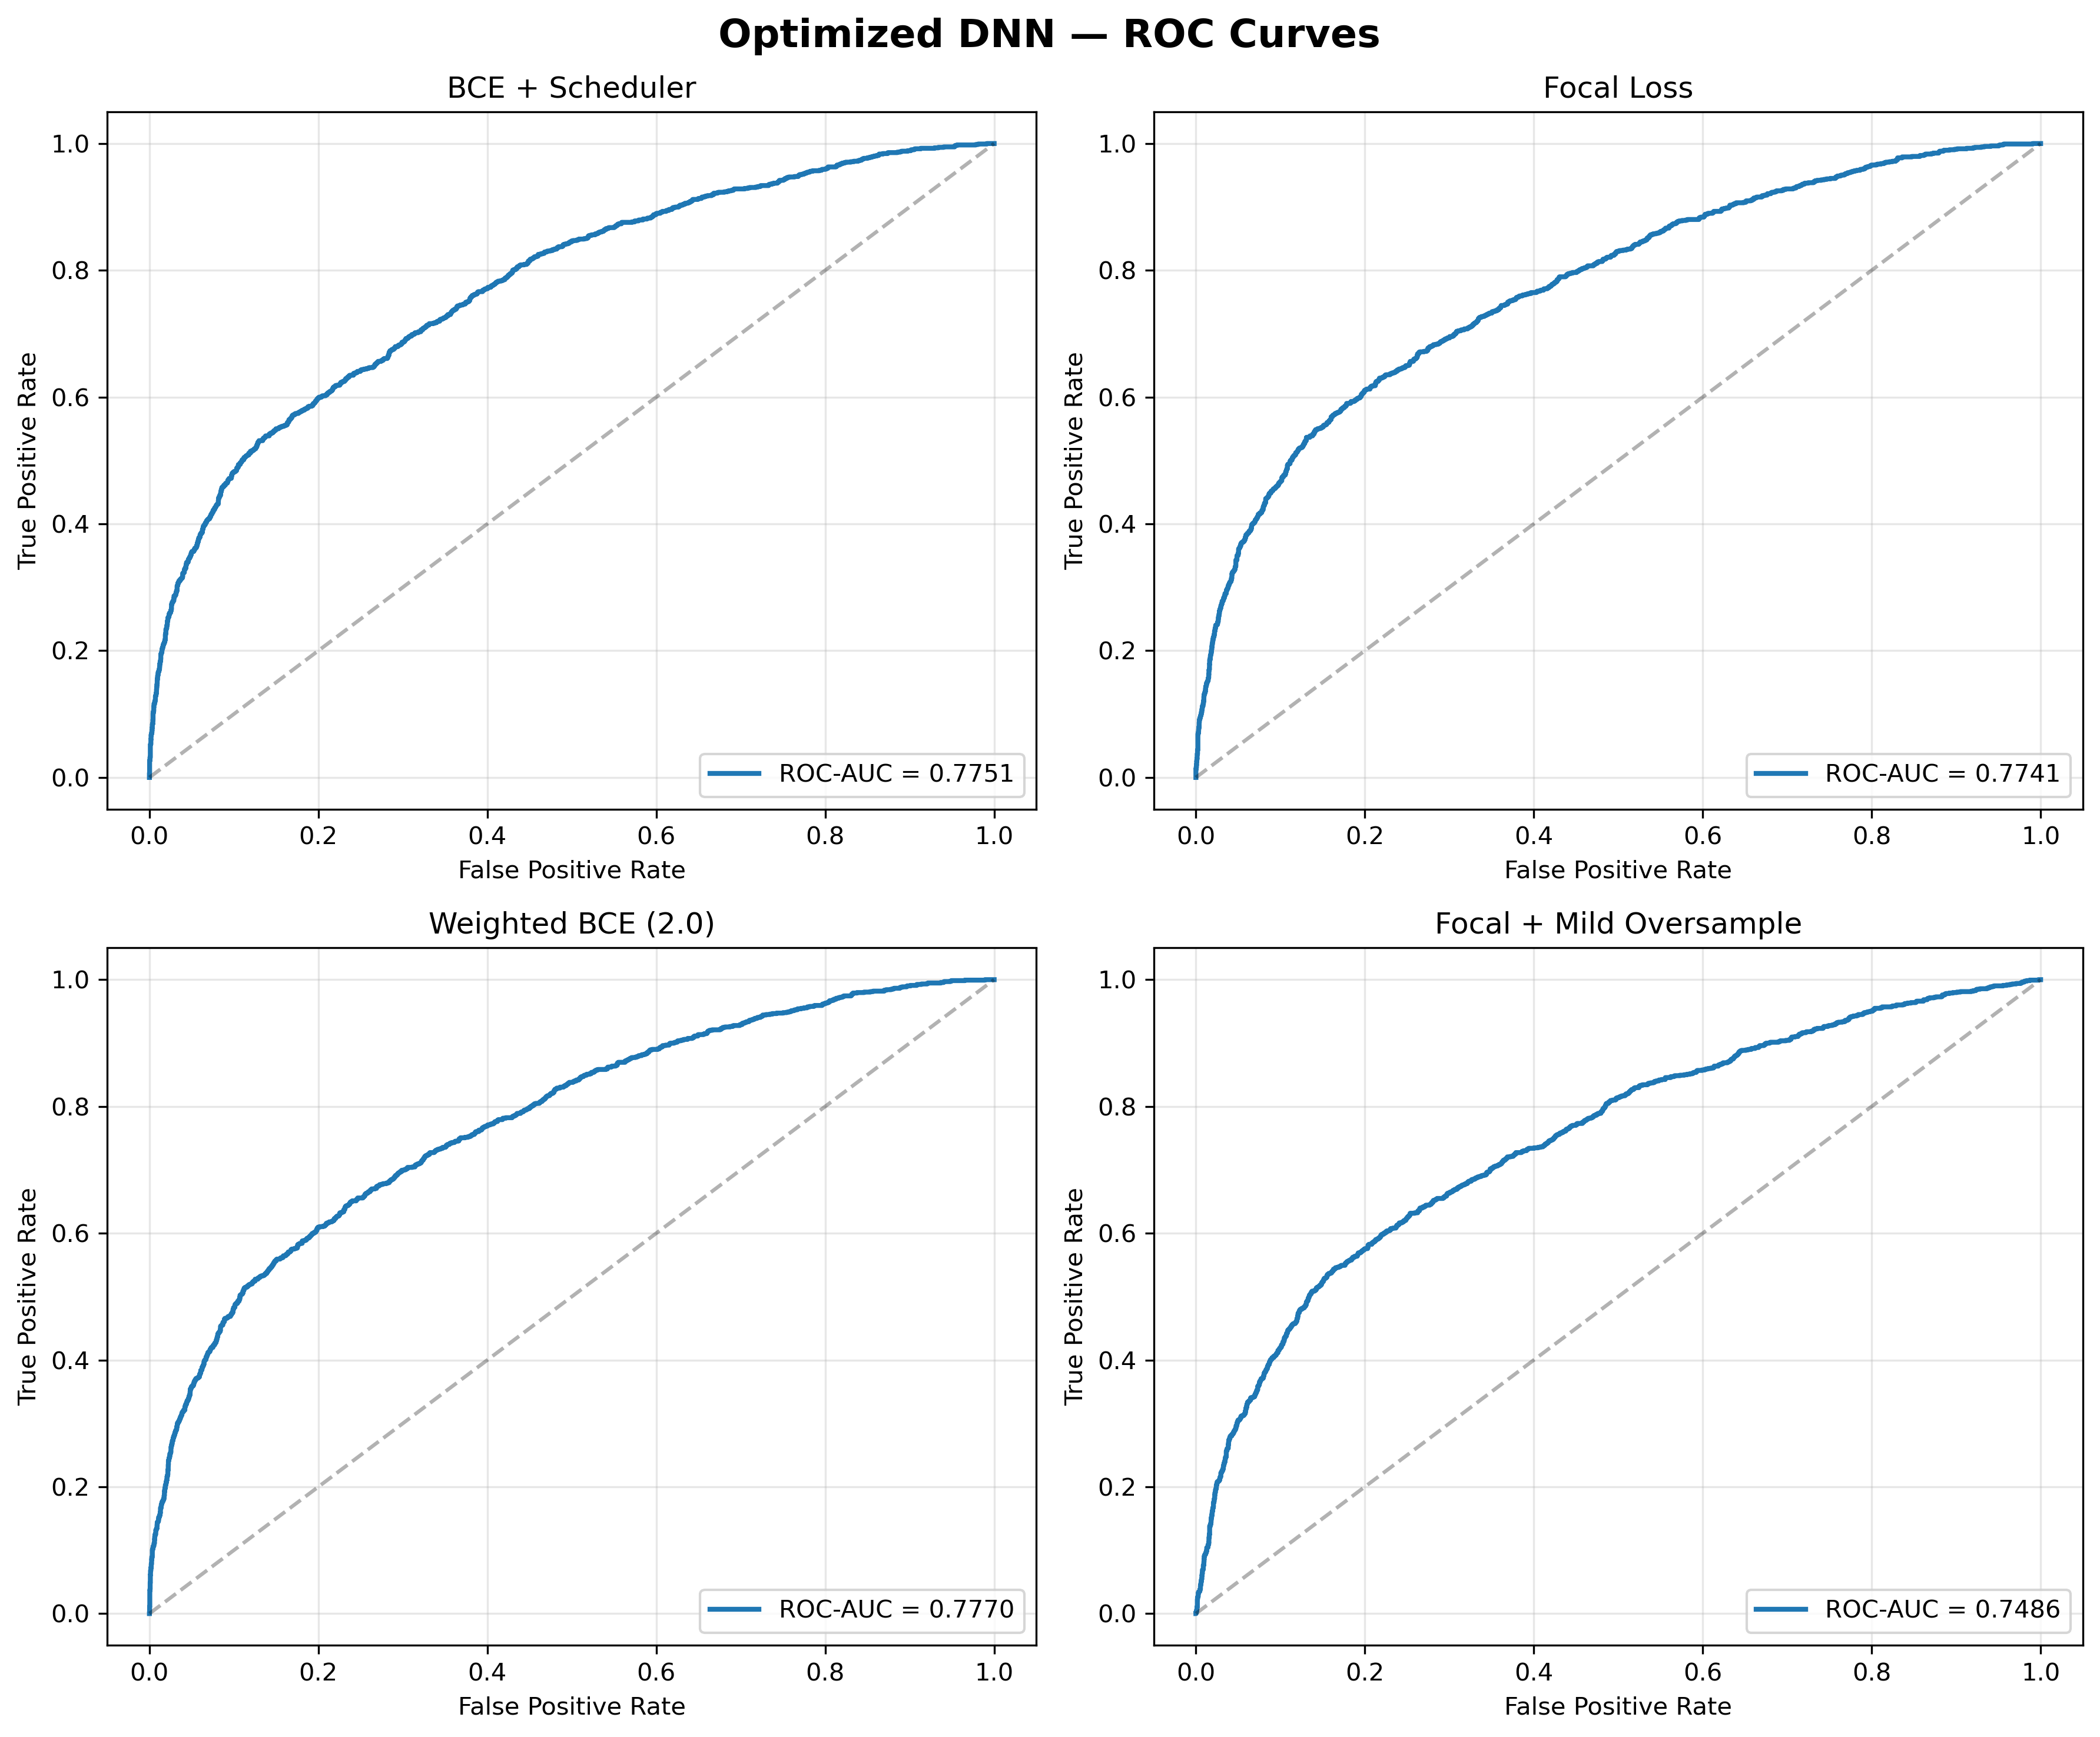
\includegraphics[width=0.48\textwidth]{30_optimized_dnn_roc.png}
    \caption{ROC curves for optimized DNN variants.}
    \label{fig:dnn_roc}
\end{figure}

\subsection{Threshold Optimization}
In risk-sensitive applications, the default decision threshold of 0.5 may not be optimal. Figure~\ref{fig:threshold} demonstrates the effect on Random Forest.

\begin{figure}[H]
    \centering
    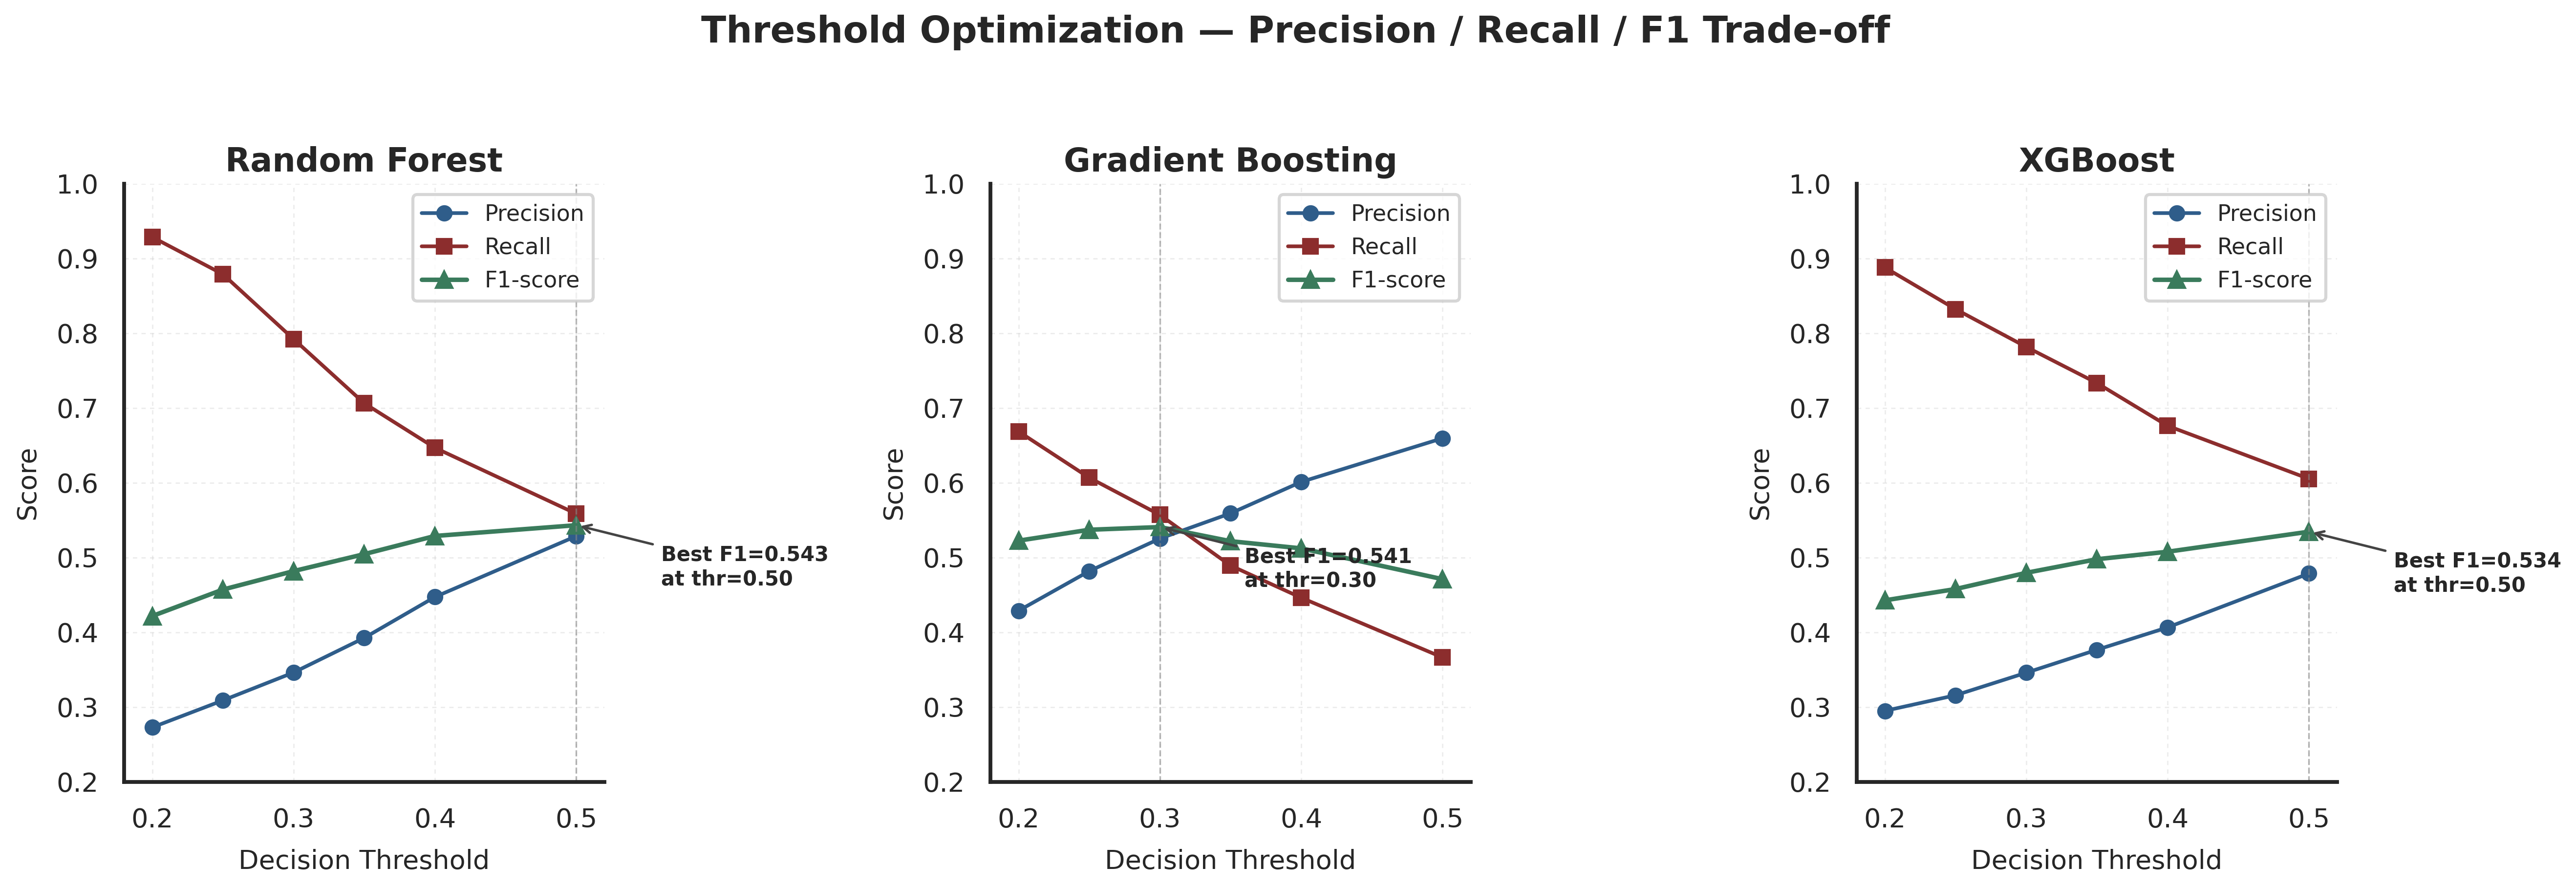
\includegraphics[width=0.48\textwidth]{25_threshold_optimization.png}
    \caption{Threshold optimization for Random Forest: lowering the threshold from 0.5 to 0.3 increases recall from 0.558 to 0.792.}
    \label{fig:threshold}
\end{figure}

\section{Discussion}

\subsection{Feature Importance}
Figure~\ref{fig:feat_imp} plots Random Forest feature importance. Repayment status variables (PAY\_0 through PAY\_6) dominate, followed by LIMIT\_BAL and engineered features such as \emph{severe\_delay\_count} and \emph{delay\_count}. This confirms that a client's repayment history is the most reliable predictor of future default, and that our engineered features successfully consolidate distributed risk signals.

\begin{figure}[H]
    \centering
    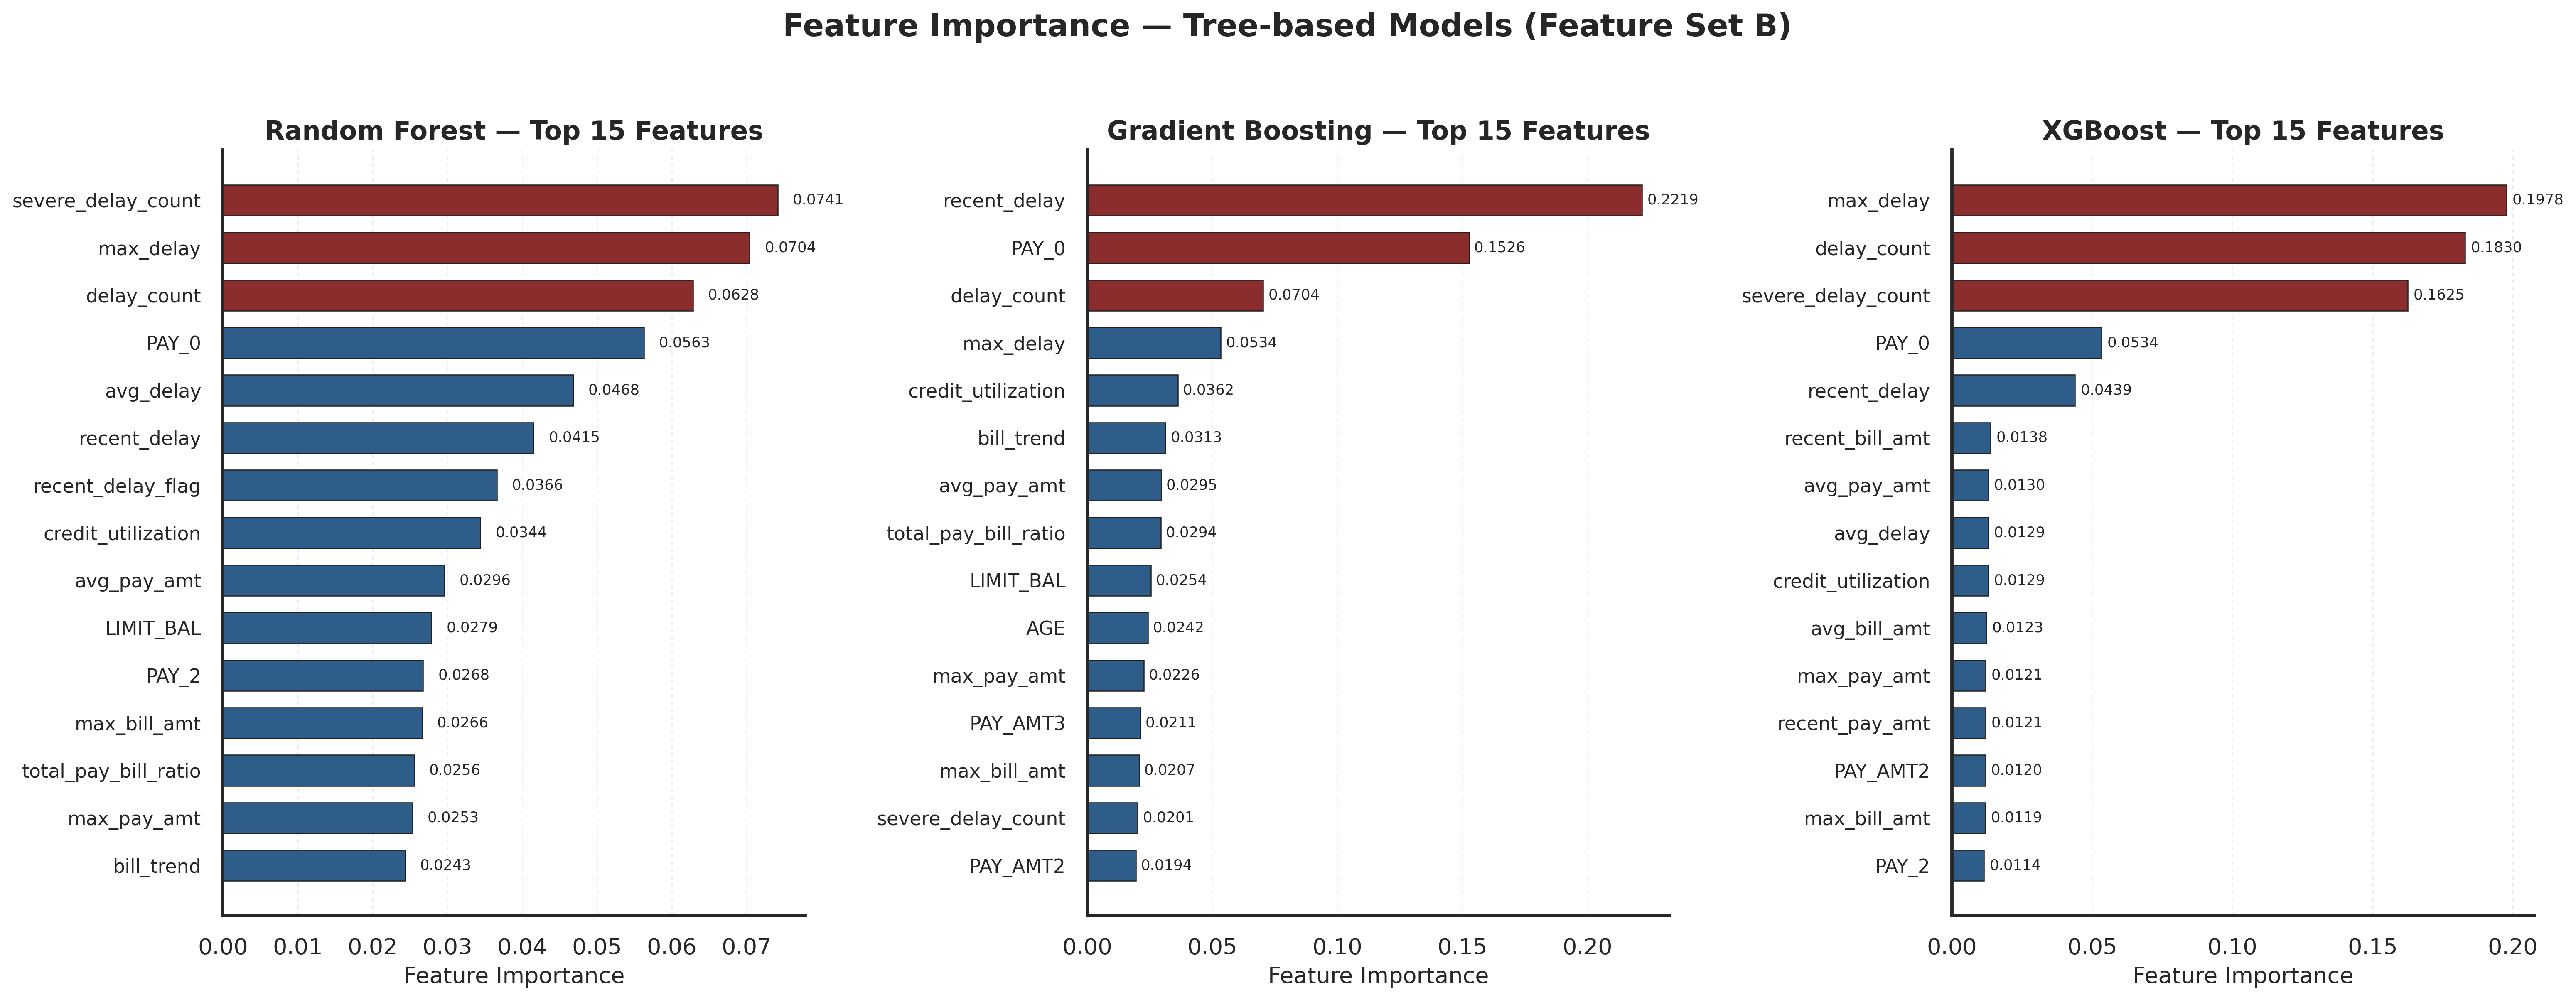
\includegraphics[width=0.48\textwidth]{27_feature_importance_tree_models.png}
    \caption{Random Forest feature importance. Repayment status variables dominate, validating the EDA findings.}
    \label{fig:feat_imp}
\end{figure}

\subsection{Implications for Risk-Sensitive Deployment}
Our results offer practical guidance:

\begin{itemize}
    \item \textbf{Balanced performance:} Random Forest or XGBoost at default threshold (0.5) suit general-purpose credit screening.
    \item \textbf{Maximizing default detection:} A threshold of 0.30--0.35 with Random Forest raises recall to 0.79, appropriate for early-warning systems.
    \item \textbf{Minimizing false positives:} Gradient Boosting or SVM achieve precision above 0.65, suitable when operational cost per alerted case is high.
\end{itemize}

\section{Conclusion and Future Work}
We presented a comprehensive machine learning framework for credit card default prediction. Through systematic feature engineering, we demonstrated that repayment-behavior features improve predictive performance across diverse classifiers. Our comparison showed that ensemble methods, particularly Random Forest and XGBoost, achieve the best performance. We further demonstrated that DNNs, with appropriate loss-function choice (Weighted BCE or Focal Loss), become competitive with ensemble methods---a 5.9~pp F1 improvement over the standard baseline.

Future work could explore: (1)~transformer-based models for temporal repayment patterns; (2)~alternative data sources beyond traditional credit bureau data; (3)~fairness-aware modeling to mitigate demographic biases; and (4)~online learning for real-time risk assessment.

\section{Data and Code Availability}
The UCI Credit Card Default dataset used in this study is publicly available through the UCI Machine Learning Repository. The code for feature engineering, model training, threshold optimization, and ensemble evaluation is open-sourced and can be accessed at: \url{https://github.com/hihihinihao/credit-card-default-prediction}.

\begin{thebibliography}{00}

\bibitem{hand2005good}
D.~J. Hand and W.~E. Henley, ``Statistical classification methods in consumer credit scoring: a review,'' \textit{J. R. Stat. Soc. Ser. A}, vol.~160, no.~3, pp.~523--541, 2005.

\bibitem{west2000neural}
D.~West, ``Neural network credit scoring models,'' \textit{Comput. Oper. Res.}, vol.~27, no.~11--12, pp.~1131--1152, 2000.

\bibitem{yeh2009comparisons}
I.-C. Yeh and C.-h. Lien, ``The comparisons of data mining techniques for the predictive accuracy of probability of default of credit card clients,'' \textit{Expert Syst. Appl.}, vol.~36, no.~2, pp.~2473--2480, 2009.

\bibitem{breiman2001random}
L.~Breiman, ``Random forests,'' \textit{Mach. Learn.}, vol.~45, no.~1, pp.~5--32, 2001.

\bibitem{chen2016xgboost}
T.~Chen and C.~Guestrin, ``XGBoost: A scalable tree boosting system,'' in \textit{Proc. 22nd ACM SIGKDD}, 2016, pp.~785--794.

\bibitem{lin2017focal}
T.-Y.~Lin, P.~Goyal, R.~Girshick, K.~He, and P.~Doll\'{a}r, ``Focal loss for dense object detection,'' in \textit{Proc. IEEE Int. Conf. Comput. Vis.}, 2017, pp.~2980--2988.

\bibitem{chawla2002smote}
N.~V.~Chawla, K.~W.~Bowyer, L.~O.~Hall, and W.~P.~Kegelmeyer, ``SMOTE: synthetic minority over-sampling technique,'' \textit{J. Artif. Intell. Res.}, vol.~16, pp.~321--357, 2002.

\bibitem{arik2021tabnet}
S.~{\"O}.~Arik and T.~Pfister, ``TabNet: Attentive interpretable tabular learning,'' in \textit{Proc. AAAI Conf. Artif. Intell.}, vol.~35, no.~8, 2021, pp.~6679--6687.

\bibitem{gorishniy2021revisiting}
Y.~Gorishniy, I.~Rubachev, V.~Khrulkov, and A.~Babenko, ``Revisiting deep learning models for tabular data,'' in \textit{Proc. Adv. Neural Inf. Process. Syst.}, vol.~34, 2021, pp.~18932--18943.

\bibitem{he2009learning}
H.~He and E.~A.~Garcia, ``Learning from imbalanced data,'' \textit{IEEE Trans. Knowl. Data Eng.}, vol.~21, no.~9, pp.~1263--1284, 2009.

\bibitem{krawczyk2016learning}
B.~Krawczyk, ``Learning from imbalanced data: open challenges and future directions,'' \textit{Prog. Artif. Intell.}, vol.~5, no.~4, pp.~221--232, 2016.

\bibitem{elkan2001foundations}
C.~Elkan, ``The foundations of cost-sensitive learning,'' in \textit{Proc. 17th Int. Joint Conf. Artif. Intell.}, 2001, pp.~973--978.

\bibitem{khandani2010customer}
A.~E.~Khandani, A.~J.~Kim, and A.~W.~Lo, ``Consumer credit-risk models via machine-learning algorithms,'' \textit{J. Bank. Finance}, vol.~34, no.~11, pp.~2767--2787, 2010.

\bibitem{kingma2015adam}
D.~P.~Kingma and J.~Ba, ``Adam: A method for stochastic optimization,'' in \textit{Proc. Int. Conf. Learn. Represent.}, 2015.

\end{thebibliography}

\end{document}
